\chapter{Réalisation}
\label{chap:realisation}

\section{Introduction}
\label{sec:realisation:intro}

Ce chapitre présente la réalisation technique du projet \projectname{}. Nous détaillons l'architecture physique et logicielle, les outils utilisés, le cycle DevSecOps mis en place, la gestion du code source, l'implémentation des différentes couches de l'application, ainsi que le déploiement.

\section{Étude technique}
\label{sec:realisation:technique}

\subsection{Architecture physique}
\label{subsec:realisation:archi-physique}

\subsubsection{Infrastructure matérielle}
\label{subsubsec:realisation:materielle}

Le projet s'appuie sur une infrastructure locale déployée sur des machines virtuelles VMware Workstation, provisionnées via Terraform. Chaque membre de l'équipe est responsable de VMs dédiées selon la répartition des services.

\begin{figure}[H]
\centering
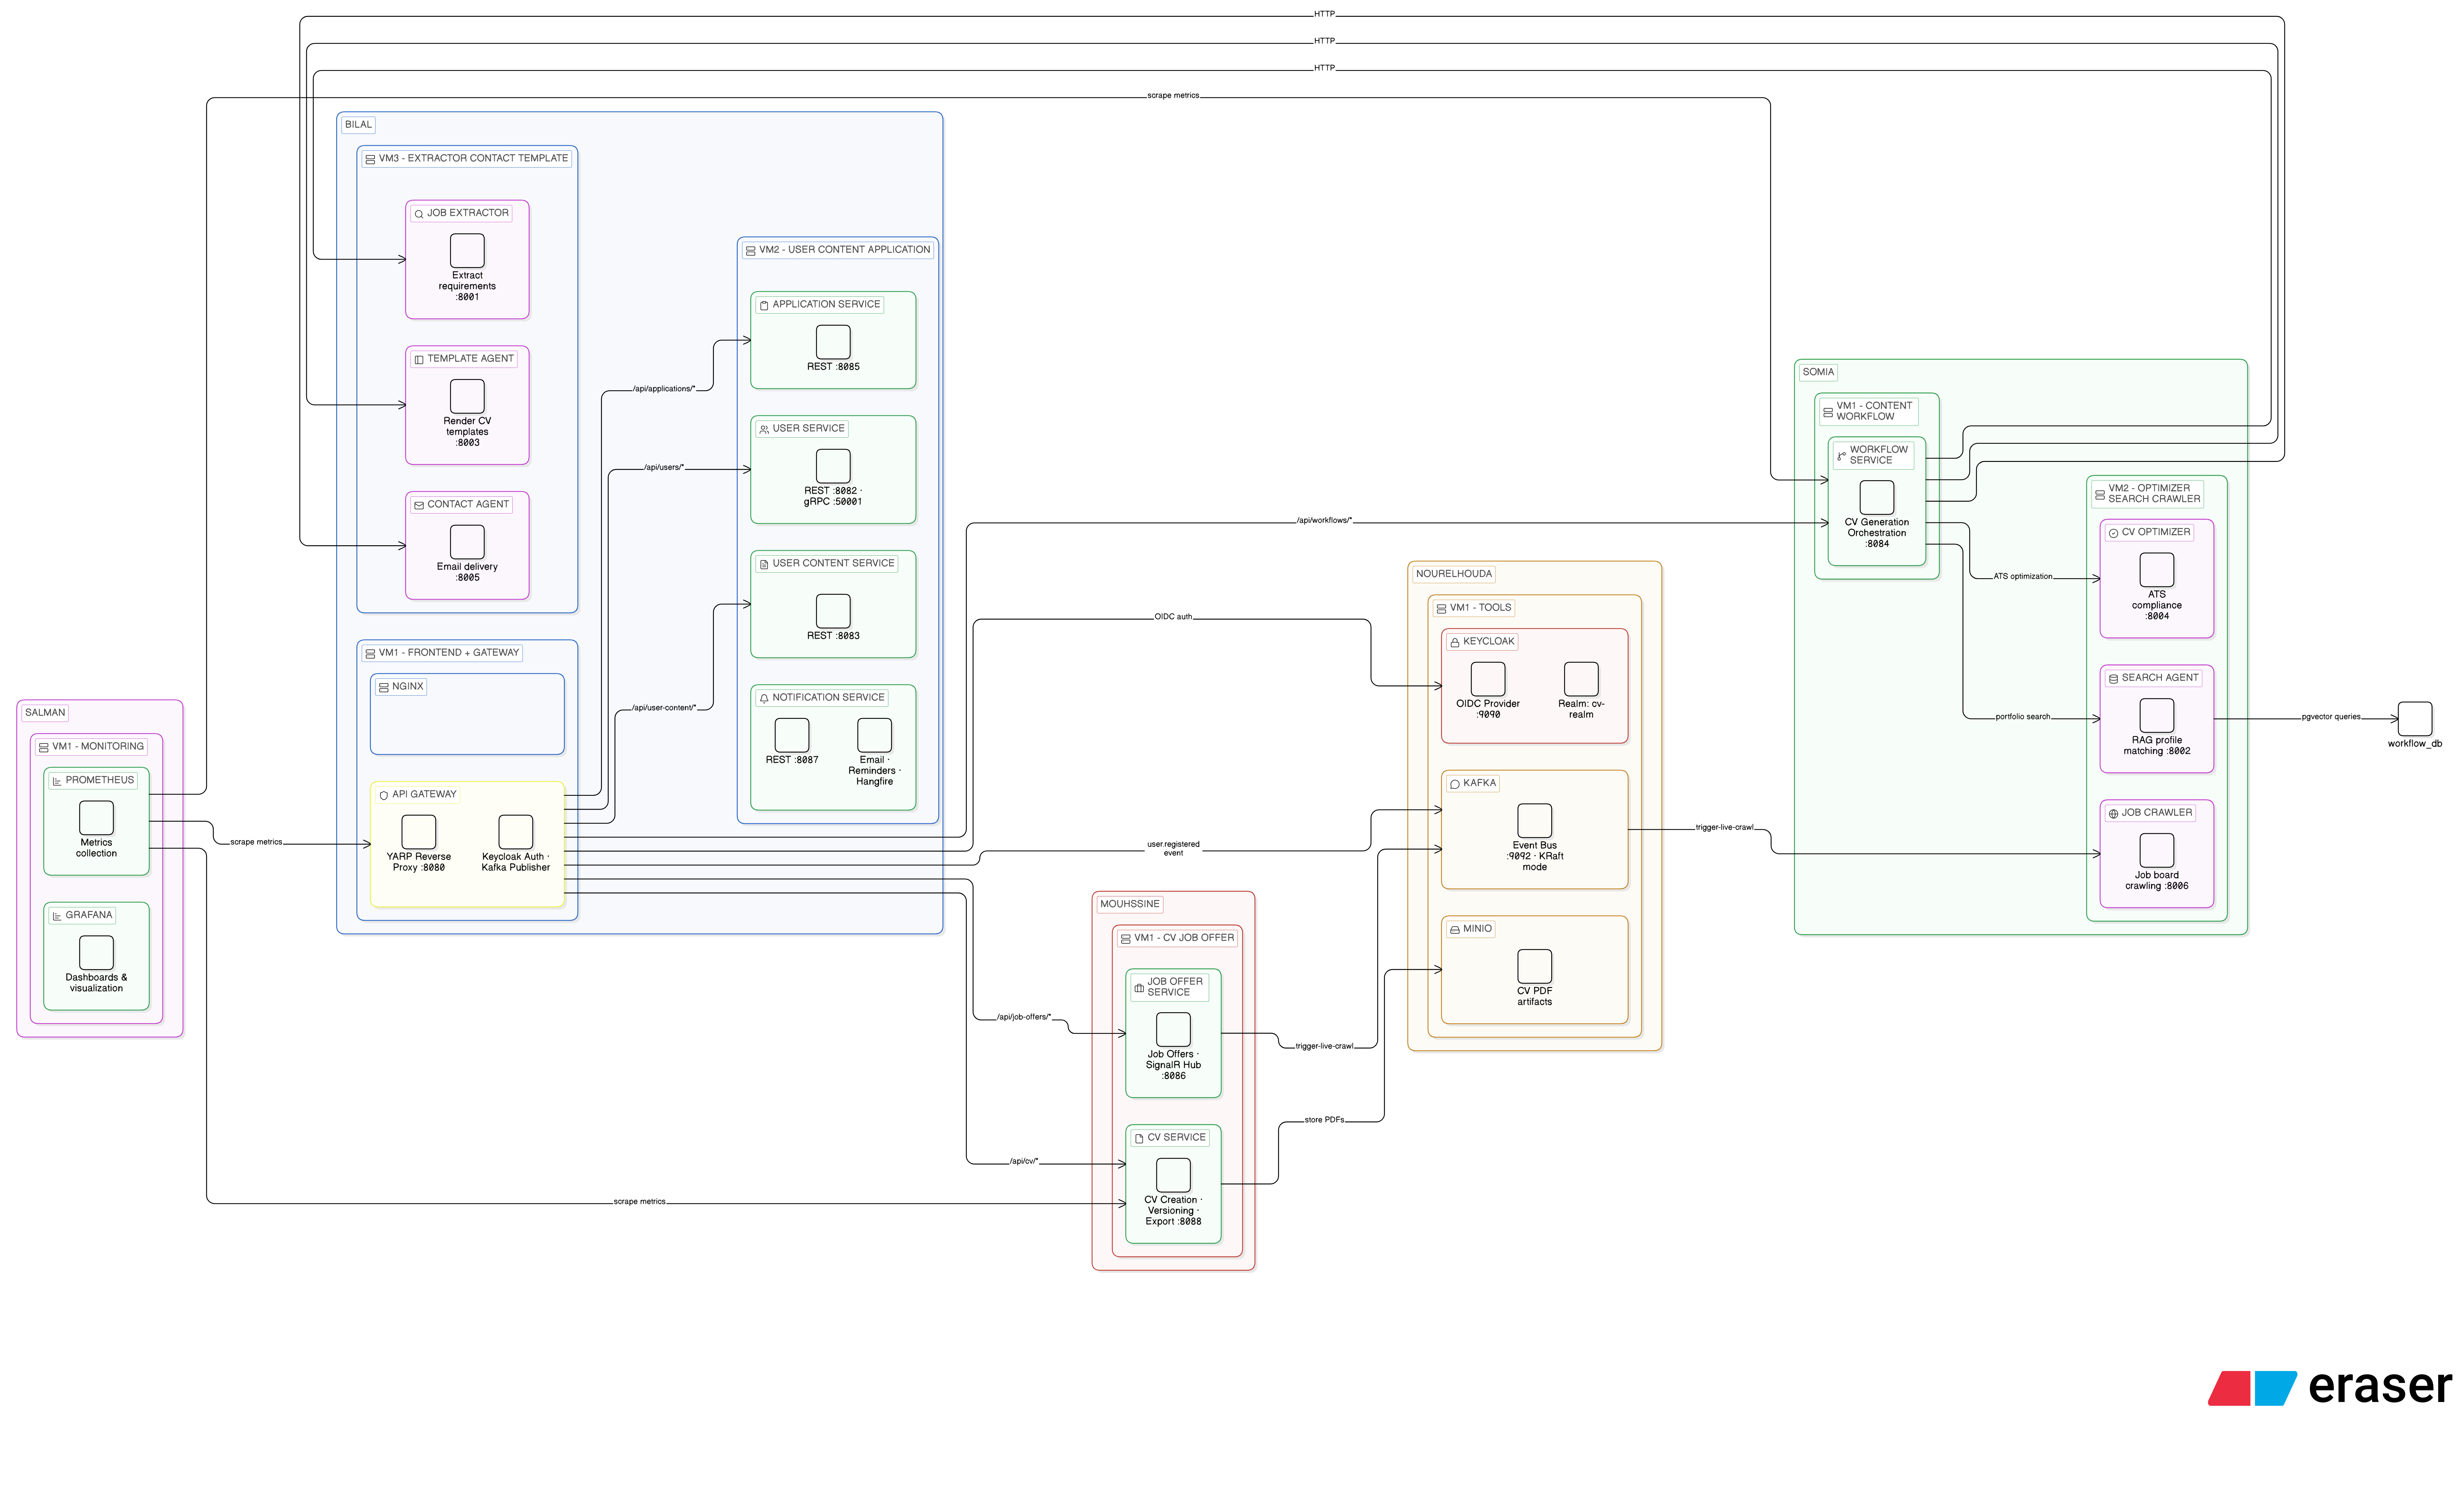
\includegraphics[width=\textwidth]{images/deployment_local.png}
\caption{Architecture de déploiement locale — Répartition des VMs par membre}
\label{fig:deployment-local}
\end{figure}

La répartition des VMs est la suivante :
\begin{itemize}
    \item \textbf{Bilal (3 VMs) :} Frontend + Gateway, Services applicatifs (User, Content, Application, Notification), Agents IA (Extractor, Contact, Template).
    \item \textbf{Somia (2 VMs) :} Service Workflow avec base pgvector, Agents IA (Optimizer, Search, Crawler).
    \item \textbf{Nourelhouda (1 VM) :} Infrastructure transverse (Keycloak, Kafka, MinIO).
    \item \textbf{Mouhssine (1 VM) :} Service CV et Service Offres d'Emploi.
    \item \textbf{Salman (1 VM) :} Monitoring (Prometheus, Grafana).
\end{itemize}

Chaque VM dispose de 2 CPU et 2 Go de RAM, et les services communiquent entre VMs via le réseau partagé Docker.

Le provisionnement des VMs est automatisé à l'aide de \textbf{Terraform} avec le provider VMware Workstation. Les scripts Terraform définissent la configuration de chaque VM (CPU, RAM, stockage) et sont versionnés dans le dépôt du projet.

\begin{figure}[H]
\centering
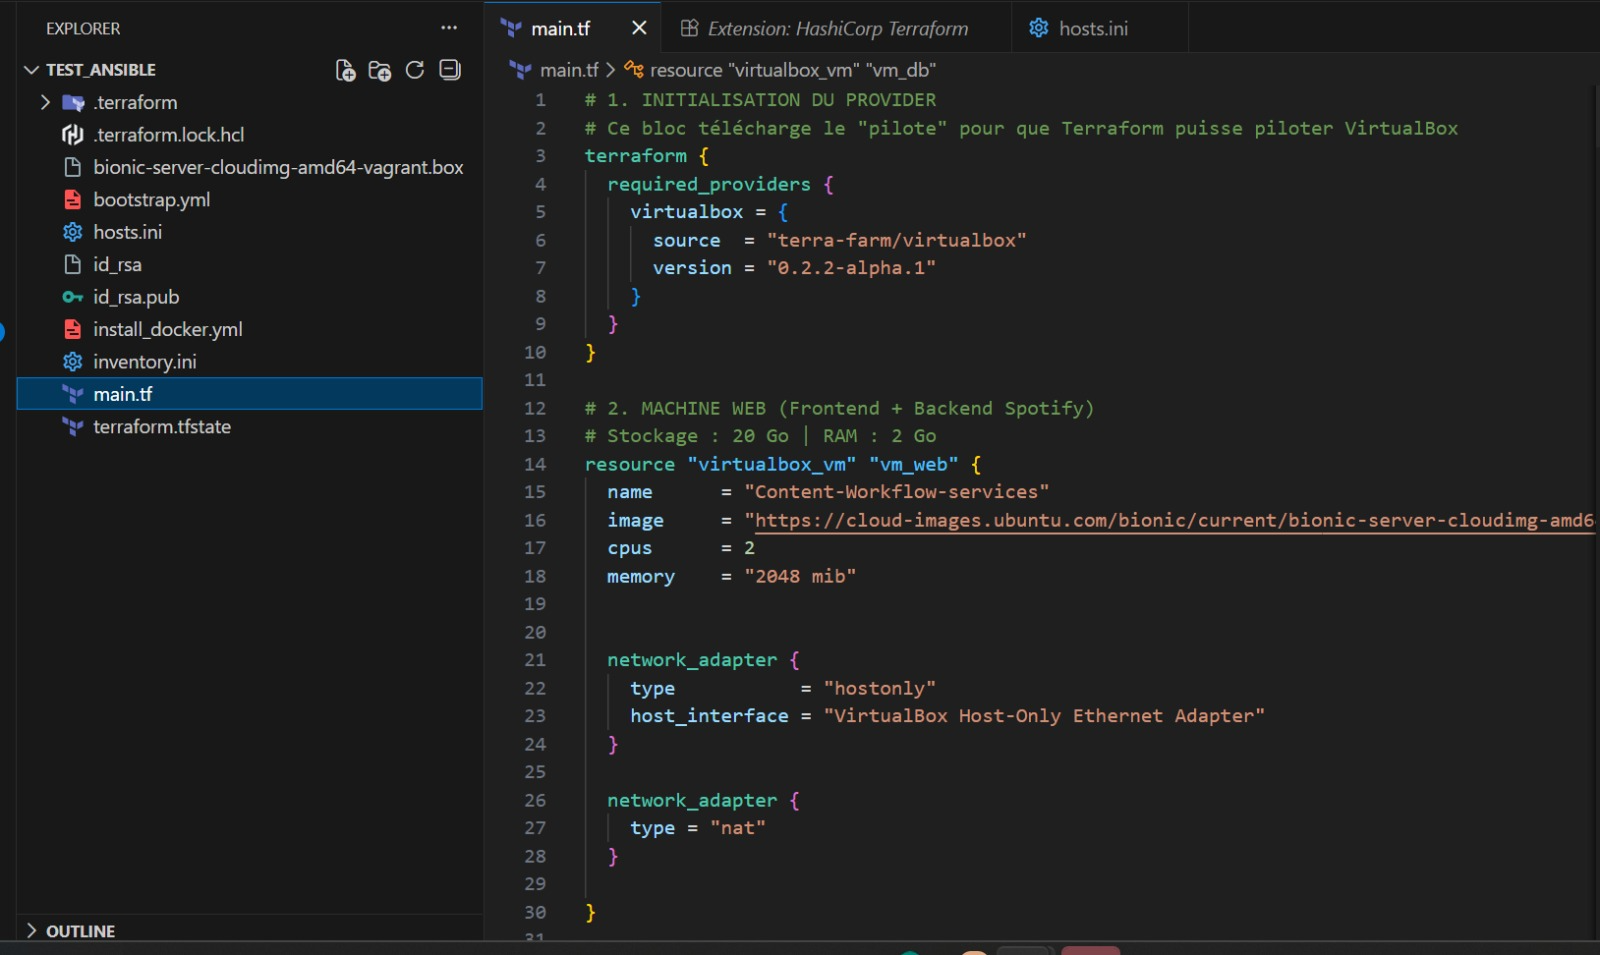
\includegraphics[width=0.85\textwidth]{images/terraform-part1.png}
\caption{Script Terraform — Définition des ressources VMs}
\label{fig:terraform-part1}
\end{figure}

\begin{figure}[H]
\centering
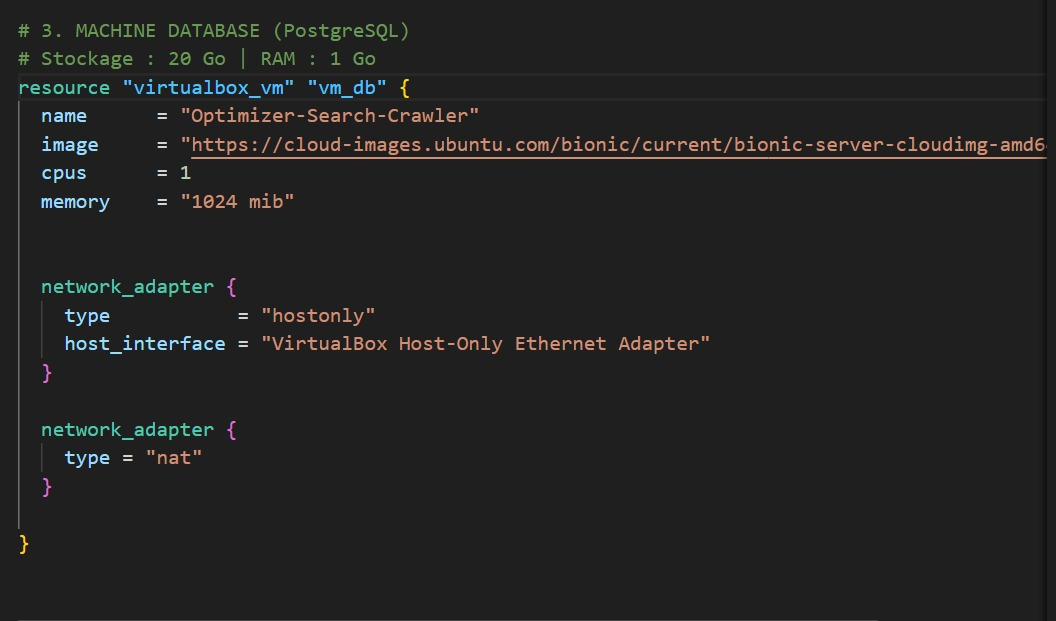
\includegraphics[width=0.85\textwidth]{images/terraform-part2.png}
\caption{Script Terraform — Configuration réseau et déploiement}
\label{fig:terraform-part2}
\end{figure}

\begin{figure}[H]
\centering
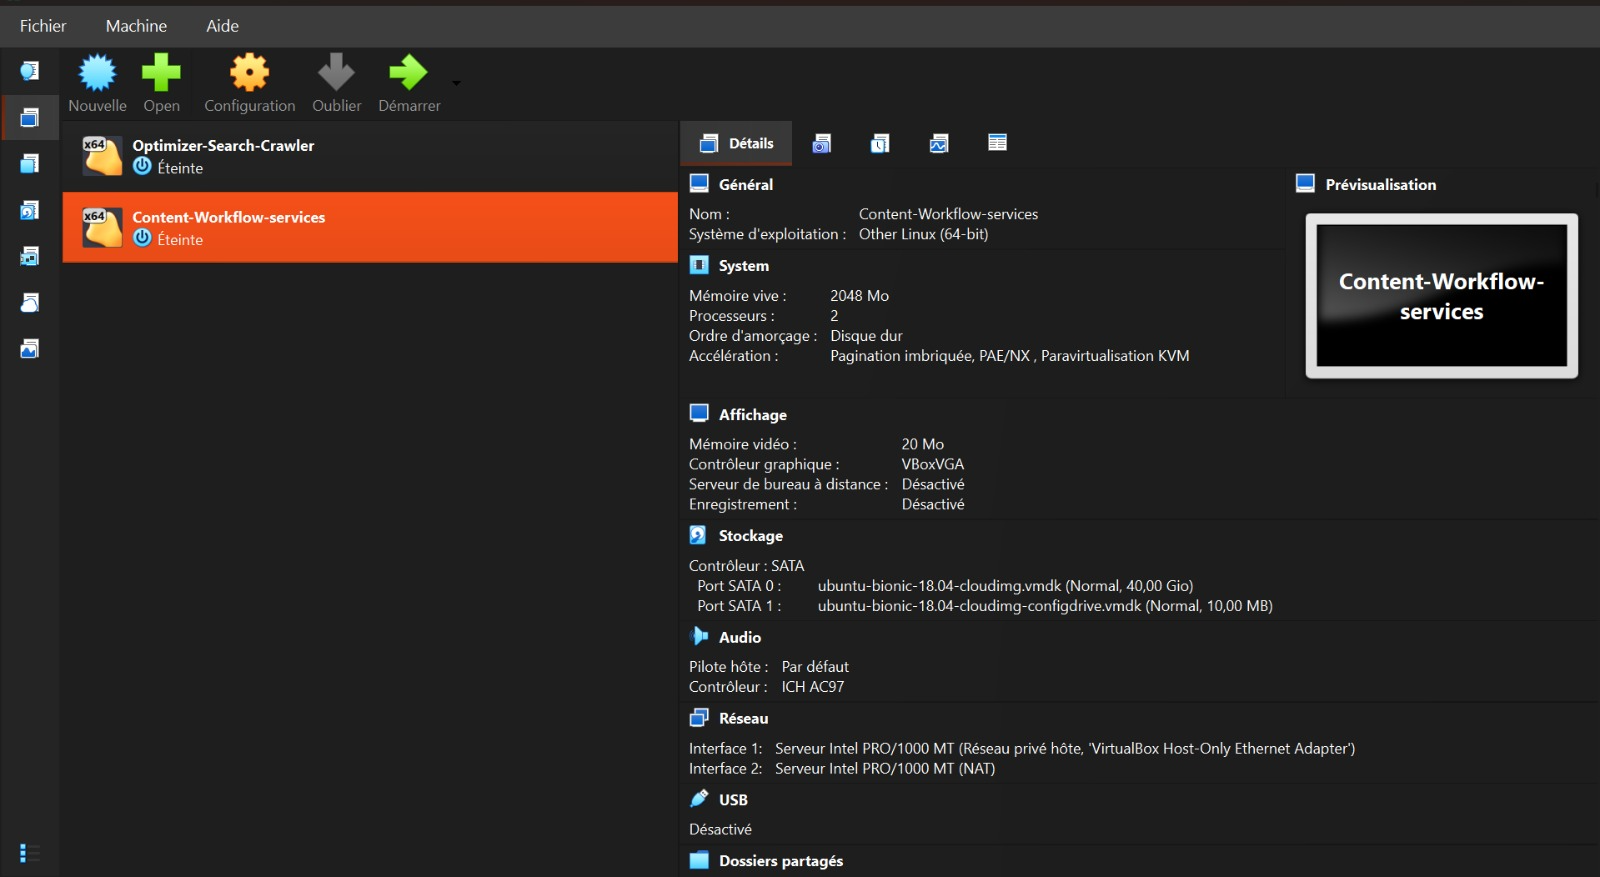
\includegraphics[width=0.85\textwidth]{images/vms-created-image-virtualbox-result.png}
\caption{Résultat du provisionnement — VMs créées}
\label{fig:vms-result}
\end{figure}

\subsubsection{Automatisation avec Ansible}
\label{subsubsec:realisation:ansible}

La configuration des VMs après provisionnement est automatisée via \textbf{Ansible}. Les playbooks Ansible installent Docker, Docker Compose, pullent les images des services et assurent la configuration réseau de chaque VM.

\begin{figure}[H]
\centering
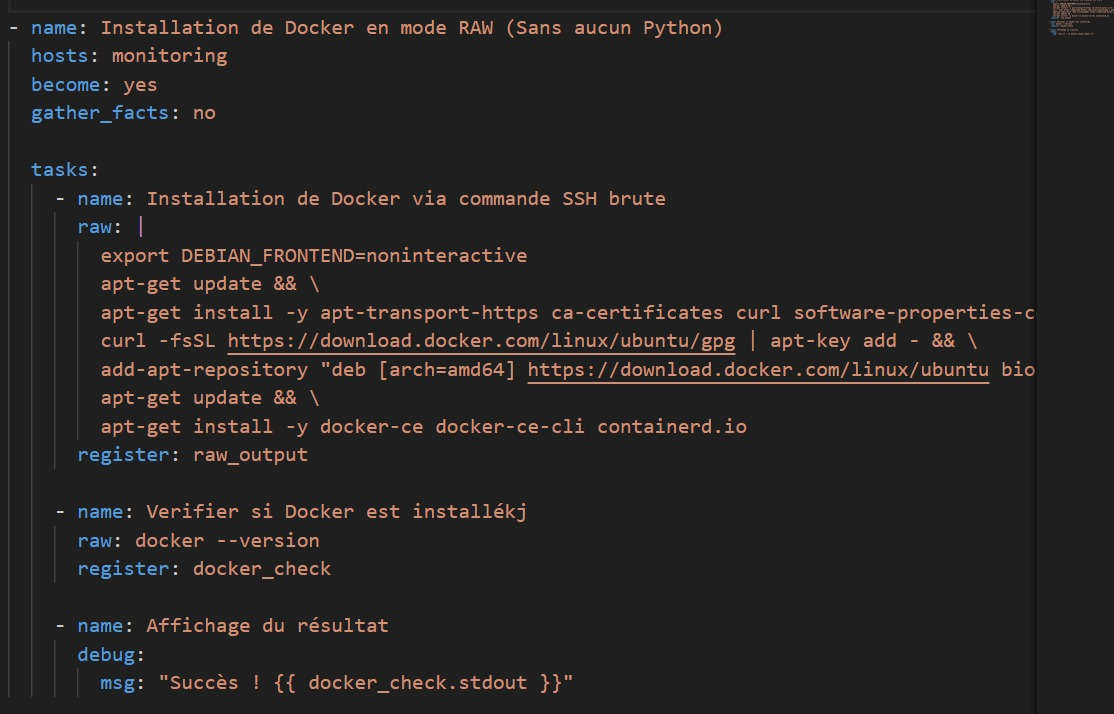
\includegraphics[width=0.85\textwidth]{images/ansible-script.png}
\caption{Playbook Ansible pour la configuration des VMs}
\label{fig:ansible-script}
\end{figure}

\begin{figure}[H]
\centering
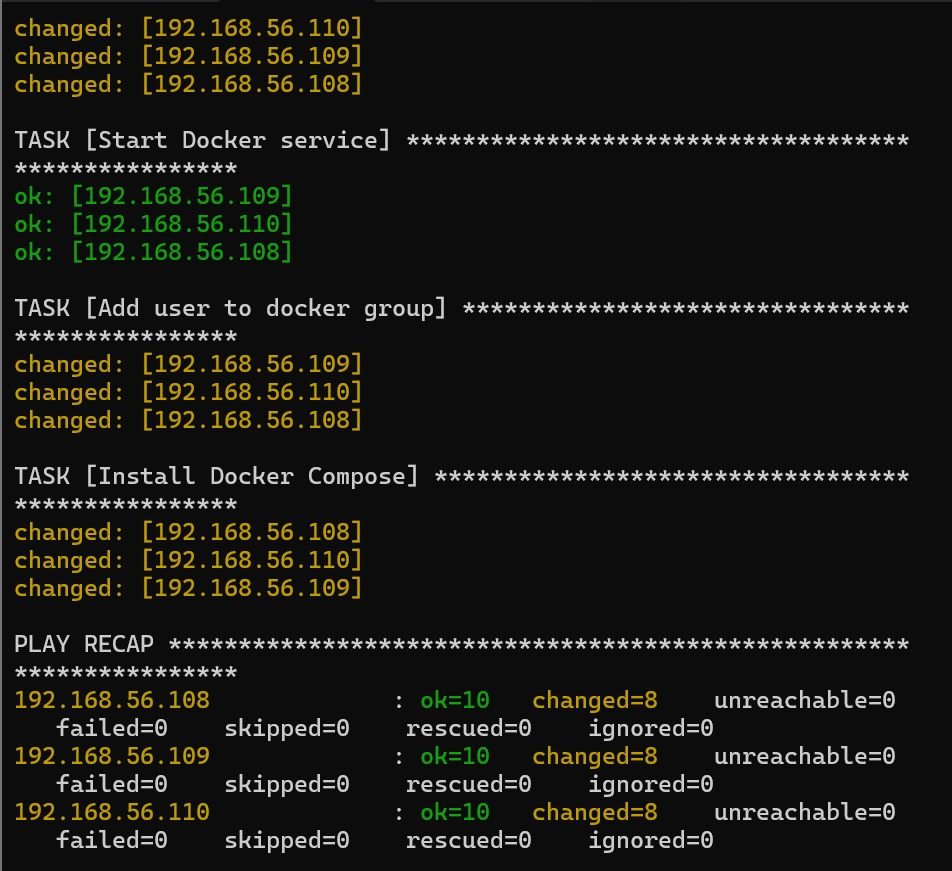
\includegraphics[width=0.85\textwidth]{images/ansible-execution-logs.png}
\caption{Logs d'exécution d'Ansible}
\label{fig:ansible-logs}
\end{figure}

\subsubsection{Infrastructure cloud}
\label{subsubsec:realisation:cloud}

\textit{Cette section sera complétée une fois l'infrastructure cloud finalisée.}

\subsubsection{Environnement de déploiement}
\label{subsubsec:realisation:deploiement}

L'ensemble de l'application est conteneurisé à l'aide de \textbf{Docker}. Chaque service possède son propre Dockerfile avec une construction multi-stage optimisée. L'orchestration est assurée par \textbf{Docker Compose} au niveau racine du projet, qui inclut trois fichiers compose spécialisés :

\begin{itemize}
    \item \textbf{backend/docker-compose.yml :} Contient les 7 microservices backend .NET, les 8 bases de données PostgreSQL, Kafka, et MinIO.
    \item \textbf{ai\_agents/docker-compose.yml :} Contient le pipeline de 6 agents IA en Python avec leur orchestrateur.
    \item \textbf{api\_gateway/docker-compose.yml :} Contient la passerelle API (YARP) et Keycloak.
\end{itemize}

Tous les services partagent un réseau Docker commun (\texttt{cv-network}) pour la communication inter-services.

\subsection{Architecture logicielle}
\label{subsec:realisation:archi-logicielle}

L'architecture logicielle de \projectname{} suit un modèle en \textbf{microservices} avec communication événementielle. Le schéma ci-dessous illustre l'architecture globale du système.

\begin{figure}[H]
\centering
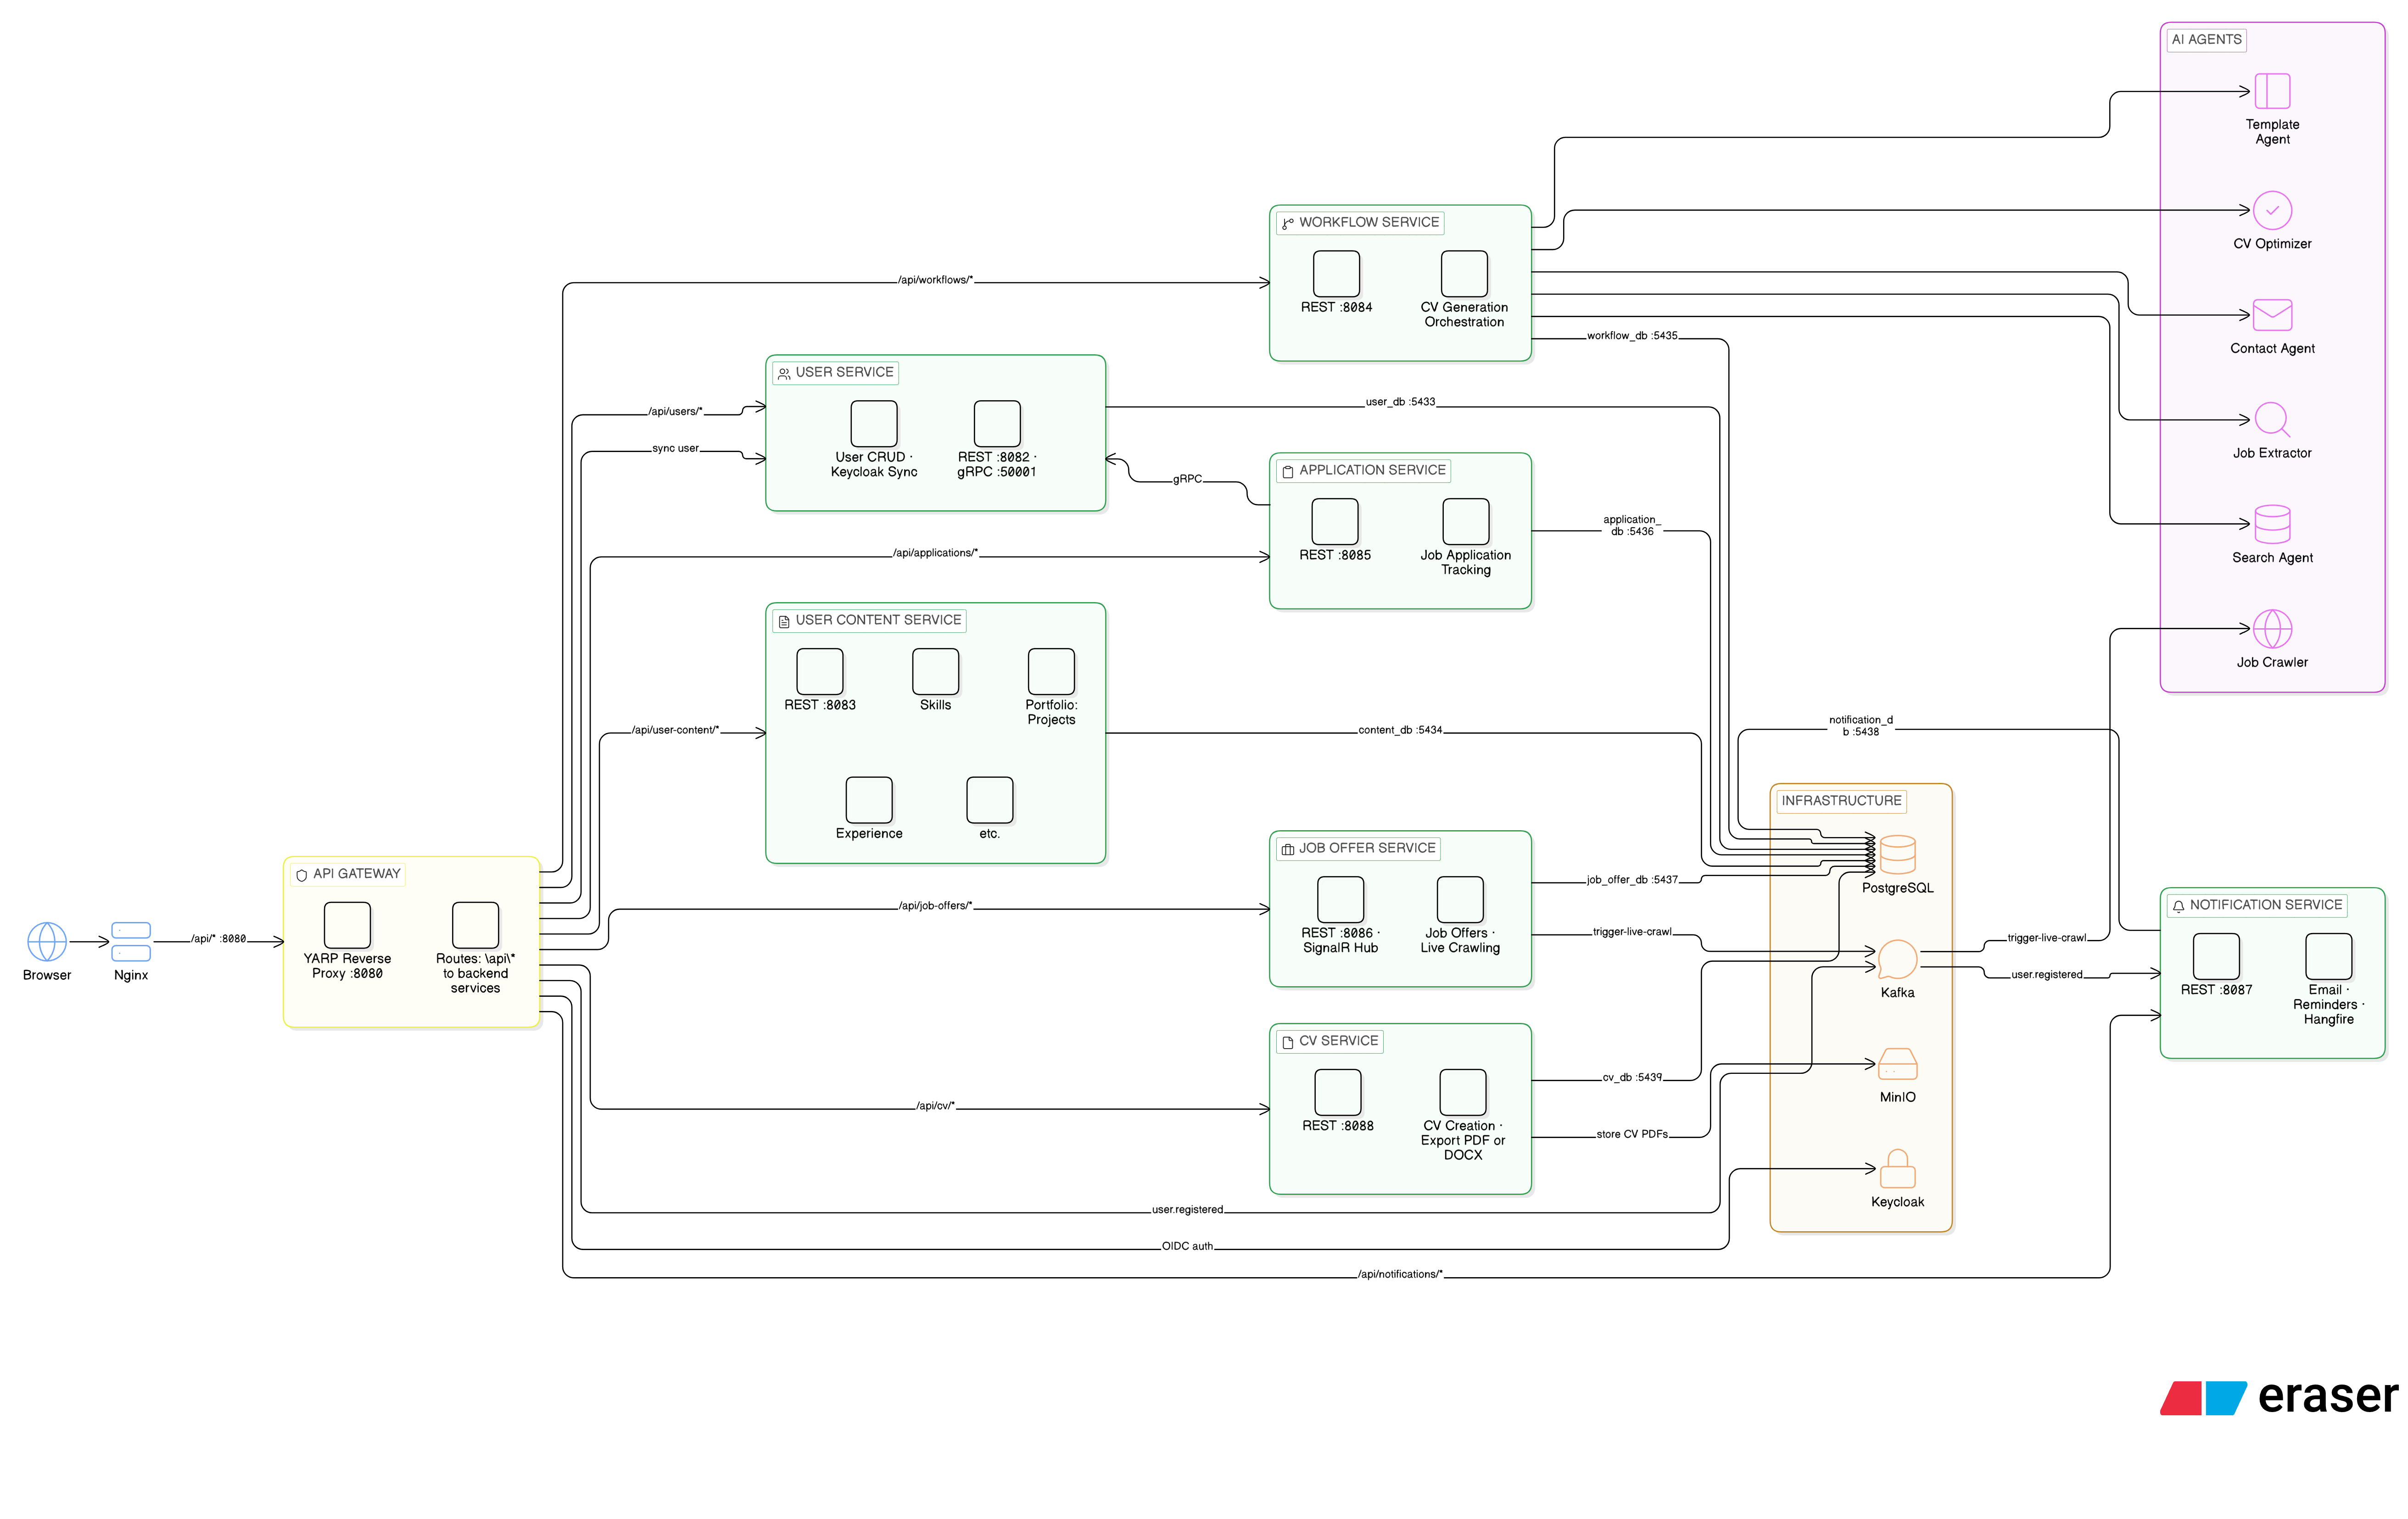
\includegraphics[width=\textwidth]{images/system-architecture.png}
\caption{Architecture logicielle du système}
\label{fig:archi-logicielle}
\end{figure}

Les sections suivantes détaillent chaque couche de l'architecture.

\subsubsection{Architecture du Frontend}
\label{subsubsec:realisation:archi-frontend}

Le frontend est une application monopage (\gls{spa}) développée avec \textbf{Angular 21} en utilisant les \textbf{standalone components}. La gestion asynchrone est assurée par \textbf{RxJS} et la réactivité par les \textbf{Signals} d'Angular. L'interface utilise le design system \textbf{Propel} avec des couleurs en espace OKLCH. L'application est hébergée par un serveur \textbf{Nginx} servant les fichiers compilés.

Le code source est organisé selon les bonnes pratiques Angular avec une séparation claire entre les \texttt{components}, \texttt{services}, \texttt{pipes} et \texttt{guards}. La structure des dossiers est présentée dans la capture ci-dessous.

\begin{figure}[H]
\centering
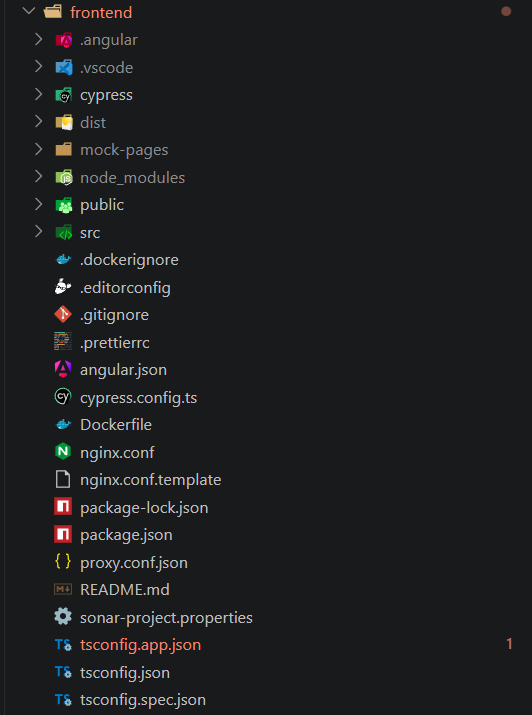
\includegraphics[width=0.7\textwidth]{images/architecture/frontend-arch.png}
\caption{Structure du projet Frontend Angular}
\label{fig:frontend-arch}
\end{figure}

\subsubsection{Passerelle API (YARP)}
\label{subsubsec:realisation:archi-gateway}

La passerelle API est un service \textbf{ASP.NET Core 10} utilisant \gls{yarp} comme proxy inverse. Elle agit comme point d'entrée unique pour toutes les requêtes clientes et assure les responsabilités suivantes :

\begin{itemize}
    \item \textbf{Routage :} Redirection des requêtes vers le microservice approprié selon l'URL.
    \item \textbf{Authentification :} Validation des tokens \gls{jwt}, gestion des sessions sécurisées par cookies.
    \item \textbf{Événements :} Publication des événements de connexion/déconnexion vers \gls{kafka}.
    \item \textbf{Sécurité :} Protection contre les attaques (\gls{xss}, injections, etc.).
\end{itemize}

\subsubsection{Architecture du Backend (Microservices .NET)}
\label{subsubsec:realisation:archi-backend}

Le backend est composé de 7 microservices indépendants développés en \textbf{ASP.NET Core 10}, chacun responsable d'un domaine métier spécifique avec sa propre base de données \textbf{PostgreSQL 16}. Cette architecture garantit un couplage faible et une évolutivité indépendante de chaque service.

La communication entre microservices s'effectue via trois protocoles complémentaires :

\begin{itemize}
    \item \textbf{\gls{rest} :} Communication synchrone pour les opérations \gls{crud} entre services.
    \item \textbf{\gls{grpc} :} Communication performante pour les échanges à faible latence (synchronisation utilisateur, récupération de détails).
    \item \textbf{\gls{kafka} :} Communication asynchrone et événementielle pour le découplage temporel entre services.
\end{itemize}

Le diagramme ci-dessous illustre les interactions entre les différents services.

\begin{figure}[H]
\centering
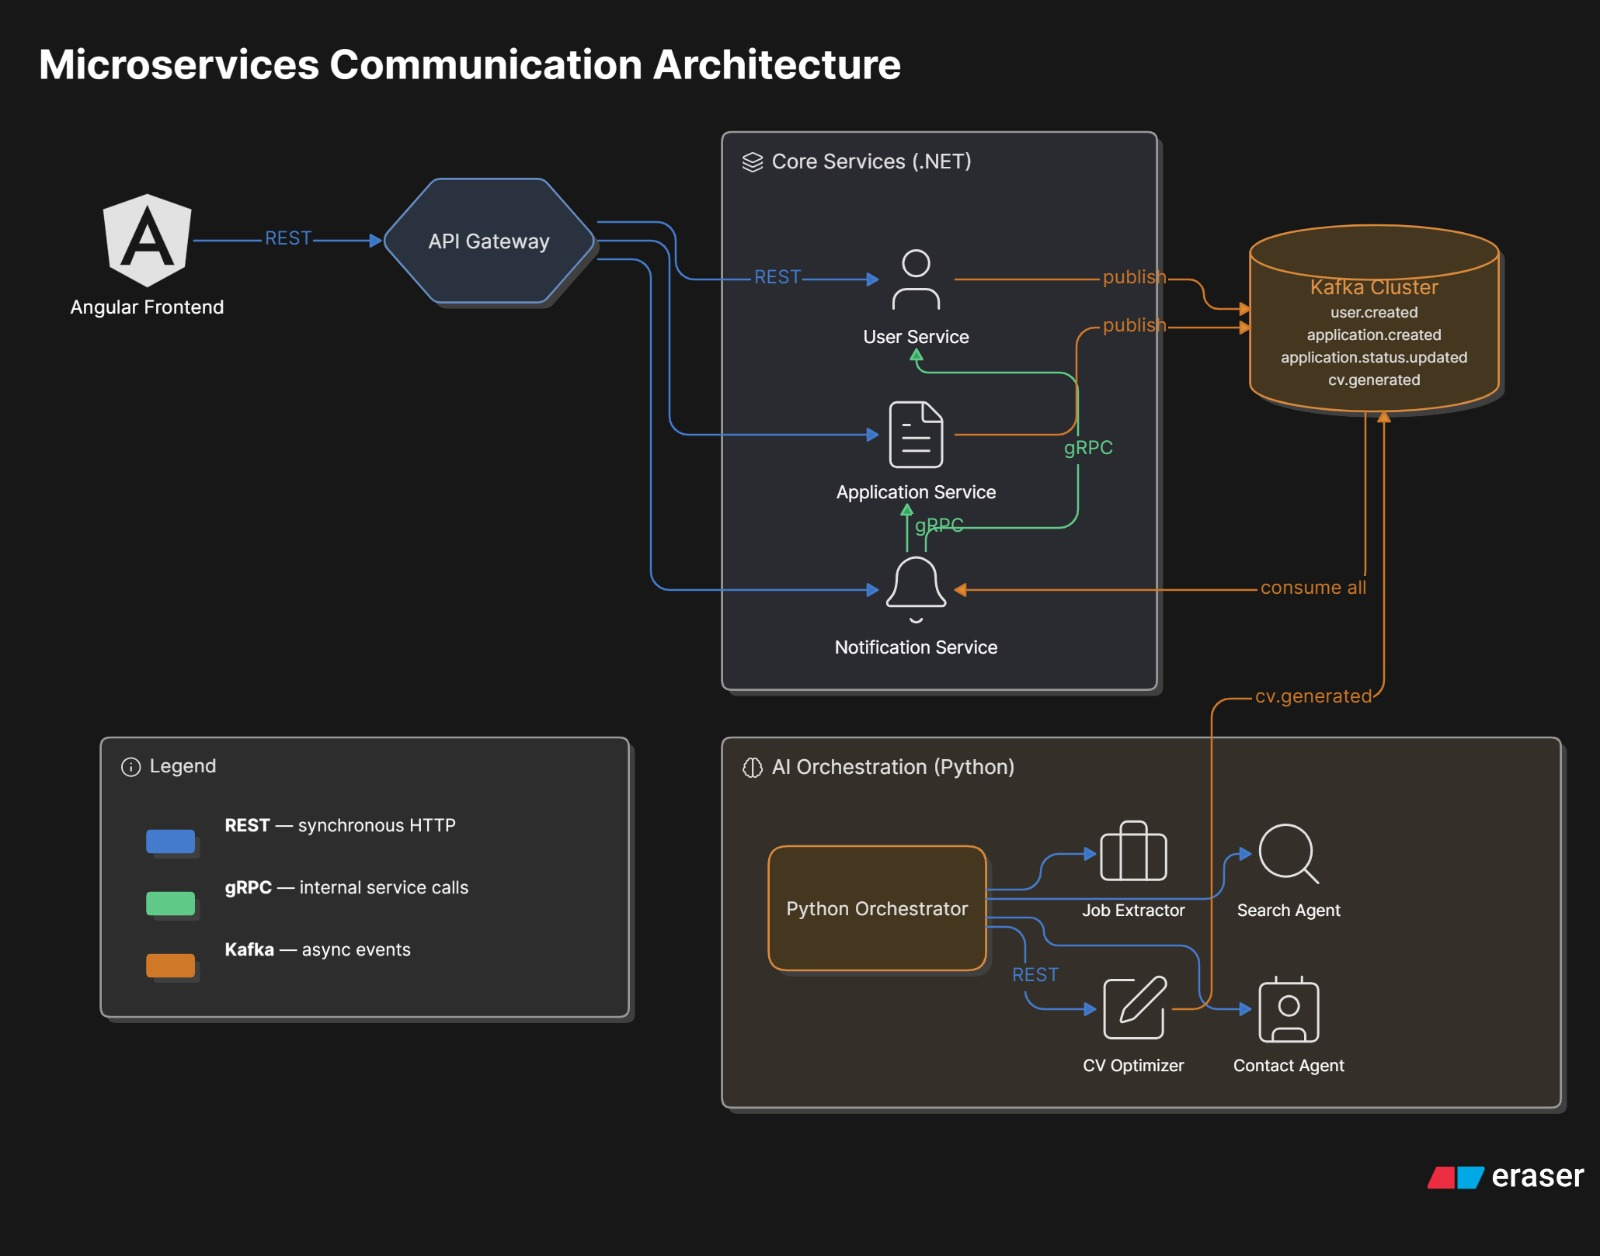
\includegraphics[width=0.9\textwidth]{images/architecture/communication-architecture.png}
\caption{Communication inter-services — \gls{rest}, \gls{grpc} et \gls{kafka}}
\label{fig:communication}
\end{figure}

La structure globale du backend est présentée ci-après.

\begin{figure}[H]
\centering
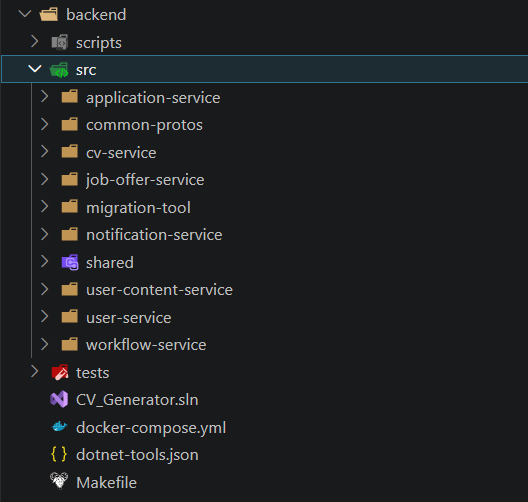
\includegraphics[width=0.8\textwidth]{images/architecture/backend-arch.png}
\caption{Structure du projet Backend \gls{dotnet}}
\label{fig:backend-arch}
\end{figure}

\paragraph{User Service}
\label{par:user-service}

Le \textbf{User Service} gère le cycle de vie des utilisateurs : inscription, authentification, mise à jour des profils et synchronisation avec \textbf{Keycloak}. Il expose une \gls{grpc} pour permettre aux autres services de récupérer les informations utilisateur. Il consomme les événements \texttt{user.registered} depuis \gls{kafka} pour créer le profil local.

\begin{figure}[H]
\centering
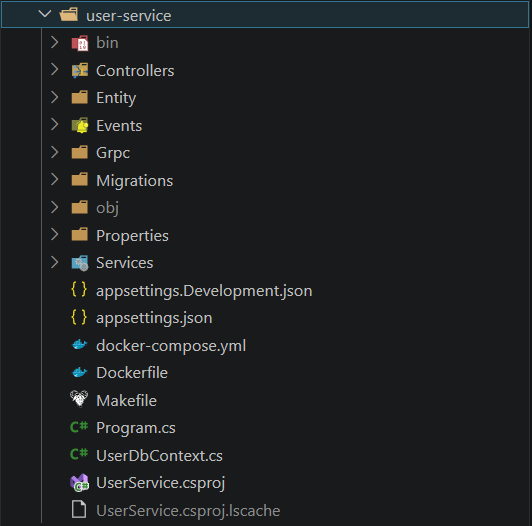
\includegraphics[width=0.65\textwidth]{images/architecture/user.png}
\caption{Structure du User Service}
\label{fig:user-service}
\end{figure}

\paragraph{User Content Service}
\label{par:user-content-service}

Le \textbf{User Content Service} gère le portfolio de l'utilisateur : projets, compétences, expériences professionnelles, formations, certifications, langues et réseaux sociaux. Il expose une \gls{rest} \gls{api} complète avec opérations \gls{crud} et est consommé par le frontend ainsi que par le \textbf{CV Service} pour la génération de CV.

\begin{figure}[H]
\centering
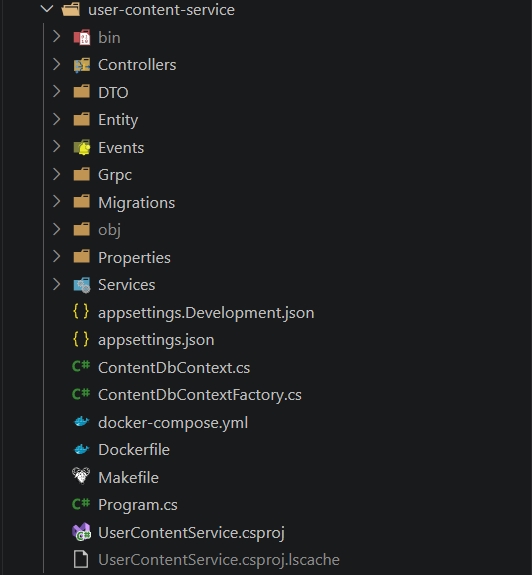
\includegraphics[width=0.65\textwidth]{images/architecture/user-contetn.png}
\caption{Structure du User Content Service}
\label{fig:user-content-service}
\end{figure}

\paragraph{CV Service}
\label{par:cv-service}

Le \textbf{CV Service} est responsable de la création, du versionnement et de l'export des CV au format \gls{pdf}. Il gère également les templates de CV et communique avec le \textbf{Workflow Service} pour déclencher les pipelines de génération. Les fichiers \gls{pdf} générés sont stockés dans \textbf{MinIO}.

\begin{figure}[H]
\centering
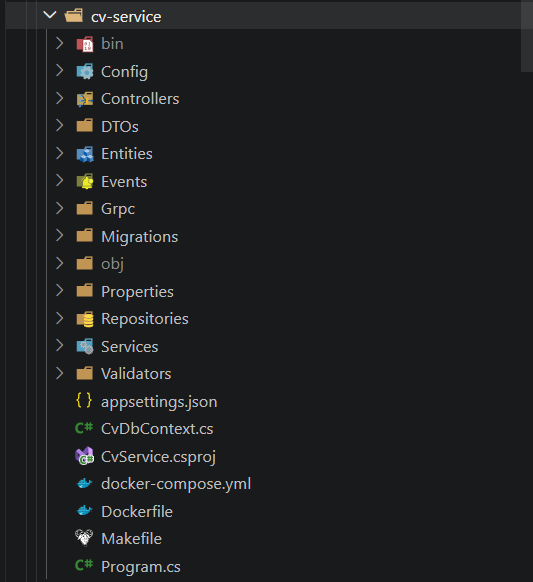
\includegraphics[width=0.65\textwidth]{images/architecture/cv.png}
\caption{Structure du CV Service}
\label{fig:cv-service}
\end{figure}

\paragraph{Workflow Service}
\label{par:workflow-service}

Le \textbf{Workflow Service} orchestre le pipeline de génération de CV. Il reçoit les demandes de génération, appelle séquentiellement les 6 agents IA via \gls{http}, et publie les résultats sur \gls{kafka}. Il utilise une base \textbf{PostgreSQL} avec l'extension \textbf{pgvector} pour le support des recherches vectorielles utilisées par l'agent de matching \gls{rag}.

\begin{figure}[H]
\centering
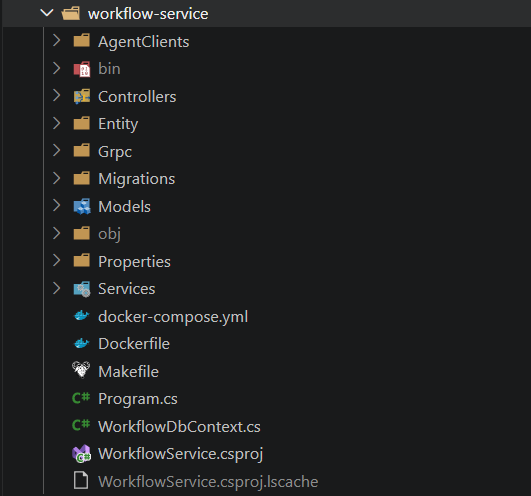
\includegraphics[width=0.65\textwidth]{images/architecture/workflow.png}
\caption{Structure du Workflow Service}
\label{fig:workflow-service}
\end{figure}

\paragraph{Application Service}
\label{par:application-service}

Le \textbf{Application Service} gère le suivi des candidatures. Il permet de créer, modifier et suivre l'état des candidatures (vue Kanban, liste, calendrier). Il communique avec le \textbf{User Service} via \gls{grpc} pour valider les utilisateurs et publie des événements de changement d'état sur \gls{kafka}.

\begin{figure}[H]
\centering
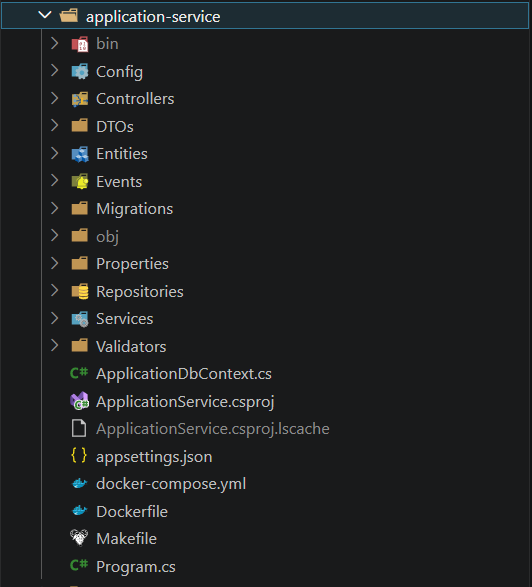
\includegraphics[width=0.65\textwidth]{images/architecture/application.png}
\caption{Structure du Application Service}
\label{fig:application-service}
\end{figure}

\paragraph{Job Offer Service}
\label{par:job-offer-service}

Le \textbf{Job Offer Service} gère les offres d'emploi. Il expose des endpoints \gls{rest} pour le \gls{crud} des offres, déclenche le crawling automatique via un agent IA dédié, et utilise \textbf{SignalR} pour les notifications temps réel vers le frontend.

\begin{figure}[H]
\centering
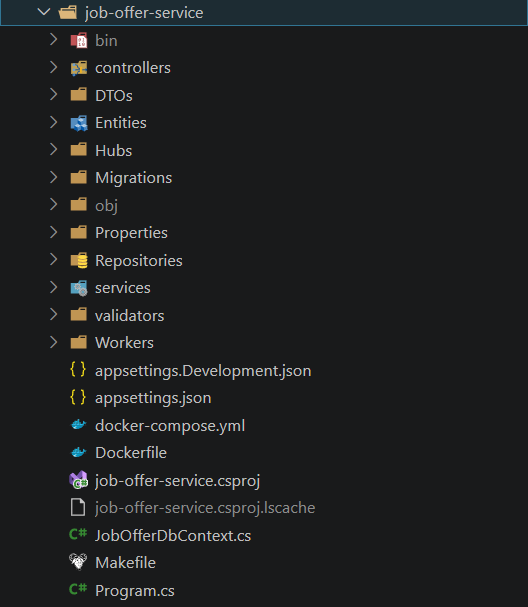
\includegraphics[width=0.65\textwidth]{images/architecture/job-offer.png}
\caption{Structure du Job Offer Service}
\label{fig:job-offer-service}
\end{figure}

\paragraph{Notification Service}
\label{par:notification-service}

Le \textbf{Notification Service} est responsable de l'envoi de notifications. Il consomme les événements \gls{kafka}, envoie des emails via \textbf{MailKit}, et gère les rappels planifiés avec \textbf{Hangfire}. Il assure la communication asynchrone avec les utilisateurs.

\begin{figure}[H]
\centering
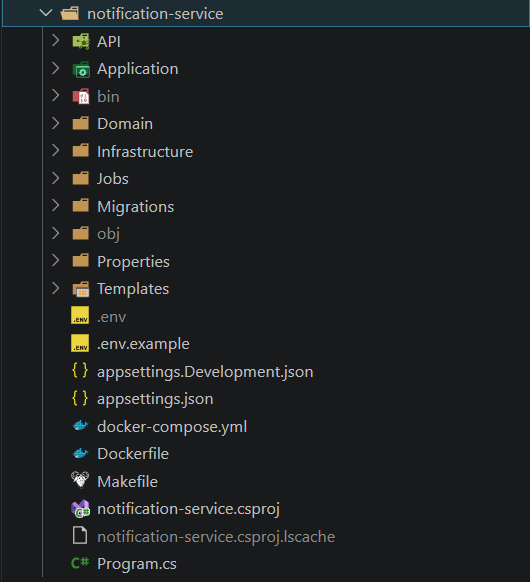
\includegraphics[width=0.65\textwidth]{images/architecture/notification.png}
\caption{Structure du Notification Service}
\label{fig:notification-service}
\end{figure}

\paragraph{Projets partagés}
\label{par:shared-projects}

En plus des 7 microservices, le backend inclut des projets partagés :

\begin{itemize}
    \item \textbf{Common :} Bibliothèque de classes partagées (DTOs, modèles, constantes) utilisée par l'ensemble des services.
    \item \textbf{Common Protos :} Définitions des contrats \gls{grpc} (fichiers \texttt{.proto}) partagés entre les services.
\end{itemize}

\begin{figure}[H]
\centering
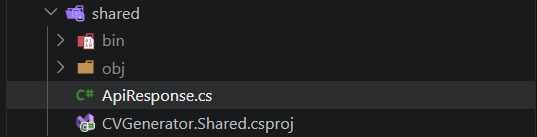
\includegraphics[width=0.5\textwidth]{images/architecture/shared.png}
\hfill
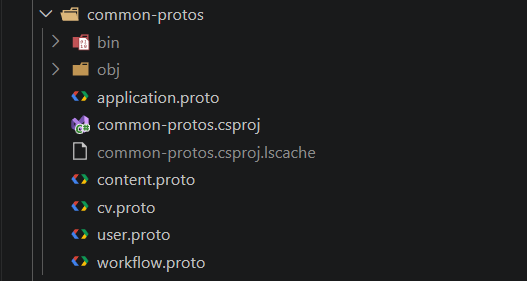
\includegraphics[width=0.45\textwidth]{images/architecture/common-protos.png}
\caption{Projets partagés — Common et Common Protos}
\label{fig:shared-projects}
\end{figure}

\subsubsection{Agents IA (Python)}
\label{subsubsec:realisation:archi-agents}

Le pipeline d'agents IA est développé en \textbf{Python} avec \textbf{FastAPI}, \textbf{LangChain} et \textbf{LangGraph}. Il se compose de 6 agents spécialisés, chacun responsable d'une étape du processus de génération de CV :

\begin{itemize}
    \item \textbf{Extractor :} Analyse l'offre d'emploi saisie par l'utilisateur et extrait les informations clés (compétences requises, expérience, formation).
    \item \textbf{Crawler :} Collecte automatiquement les offres d'emploi depuis des plateformes externes.
    \item \textbf{Search :} Recherche les meilleures correspondances dans le portfolio de l'utilisateur.
    \item \textbf{Optimizer :} Applique les techniques d'optimisation \gls{ats} pour maximiser la compatibilité du CV avec les systèmes de recrutement.
    \item \textbf{Template :} Sélectionne et applique le template de CV le plus adapté au profil et au secteur visé.
    \item \textbf{Contact :} Génère une lettre de motivation personnalisée adaptée à l'offre ciblée.
\end{itemize}

L'orchestrateur, intégré au \textbf{Workflow Service}, coordonne l'exécution séquentielle de ces agents et gère le flux de données entre chaque étape.

\subsubsection{Infrastructure transverse}
\label{subsubsec:realisation:archi-infra}

L'infrastructure transverse regroupe les services communs à l'ensemble de l'application :

\begin{itemize}
    \item \textbf{\gls{kafka} (mode KRaft) :} Système de messagerie asynchrone pour la communication événementielle. Il permet le découplage temporel entre les services et alimente le pipeline de génération de CV.
    \item \textbf{MinIO (\gls{s3}) :} Stockage d'objets compatible Amazon \gls{s3} pour les fichiers \gls{pdf} de CV générés et les templates.
    \item \textbf{Keycloak :} Serveur d'authentification centralisé supportant \gls{oauth} 2.0 et \gls{oidc}. Il gère les identités des utilisateurs et propose la fédération d'identités (Google, GitHub).
    \item \textbf{PostgreSQL 16 :} 8 bases de données indépendantes (une par microservice + une pour Keycloak), chacune avec l'extension \textbf{pgvector} pour les recherches vectorielles.
\end{itemize}

\subsection{Présentation des outils utilisés}
\label{subsec:realisation:outils}

\subsubsection{Outils de développement}
\label{subsubsec:realisation:outils-dev}

Le tableau suivant récapitule les principaux outils et technologies utilisés pour le développement :

\begin{table}[H]
\centering
\caption{Outils de développement}
\label{tab:outils-dev}
\begin{tabularx}{\textwidth}{lX}
\toprule
\textbf{Couche} & \textbf{Technologies} \\
\midrule
Frontend & Angular 21, TypeScript, RxJS, Signals, SCSS, Vitest, Cypress \\
Backend & ASP.NET Core 10, Entity Framework Core, gRPC, YARP, Hangfire, MailKit \\
Agents IA & Python, FastAPI, LangChain, LangGraph, LangChain-Groq, Pydantic \\
Bases de données & PostgreSQL 16 avec extension pgvector \\
Authentification & Keycloak 26, OpenID Connect, JWT \\
Messagerie & Apache Kafka (KRaft mode) \\
Stockage & MinIO (API S3) \\
Conteneurisation & Docker, Docker Compose \\
\bottomrule
\end{tabularx}
\end{table}

\subsubsection{Outils d'intégration et de déploiement continu (CI/CD)}
\label{subsubsec:realisation:outils-cicd}

\begin{table}[H]
\centering
\caption{Outils CI/CD et qualité}
\label{tab:outils-cicd}
\begin{tabularx}{\textwidth}{lX}
\toprule
\textbf{Outil} & \textbf{Rôle} \\
\midrule
GitHub Actions & Pipeline CI/CD (6 phases) \\
SonarCloud & Analyse statique de code et quality gates \\
Trivy & Scan de vulnérabilités (système de fichiers et images Docker) \\
OWASP ZAP & Tests de sécurité DAST (Dynamic Application Security Testing) \\
Docker & Conteneurisation multi-stage \\
GitHub Container Registry & Registre d'images Docker \\
DockerHub & Registre d'images secondaire \\
\bottomrule
\end{tabularx}
\end{table}

\section{Cycle DevSecOps}
\label{sec:realisation:devsecops}

\subsection{Présentation et importance dans le projet}
\label{subsec:realisation:devsecops-presentation}

Le cycle DevSecOps intègre la sécurité à chaque étape du cycle de développement logiciel. Dans le cadre de \projectname{}, cette approche est essentielle étant donné la nature sensible des données traitées (informations personnelles des utilisateurs, CV, données de connexion).

L'adoption du cycle DevSecOps nous permet de :
\begin{itemize}
    \item Détecter les vulnérabilités tôt dans le cycle de développement.
    \item Automatiser les contrôles de sécurité.
    \item Garantir la conformité aux bonnes pratiques.
    \item Assurer une traçabilité complète des modifications.
\end{itemize}

\subsection{Outils DevSecOps utilisés}
\label{subsec:realisation:devsecops-outils}

\begin{itemize}
    \item \textbf{SonarCloud :} Analyse statique de code avec quality gates pour les projets Angular, .NET et Python. Des seuils de qualité (couverture de code, dette technique, duplication) doivent être respectés.
    \item \textbf{Trivy :} Scan de vulnérabilités sur le système de fichiers lors des phases statiques et sur les images Docker construites. Détection des dépendances obsolètes et des failles de sécurité connues.
    \item \textbf{OWASP ZAP :} Tests DAST (Dynamic Application Security Testing) en environnement d'intégration pour détecter les vulnérabilités applicatives (XSS, injection SQL, etc.).
\end{itemize}

\subsection{Application du cycle DevSecOps dans le projet}
\label{subsec:realisation:devsecops-application}

Le cycle DevSecOps est appliqué à travers le pipeline CI/CD en six phases :

\begin{enumerate}
    \item \textbf{Phase 1 - Static Checks :} Validation des fichiers Docker Compose, scan Trivy filesystem, analyse SonarCloud pour le frontend, le backend et les agents IA.
    \item \textbf{Phase 2 - Component Tests :} Exécution des tests unitaires (.NET avec xUnit, Angular avec Vitest, Python avec pytest) et génération des rapports de couverture.
    \item \textbf{Phase 3 - Integration / E2E :} Tests d'intégration et tests E2E avec Cypress, suivis d'un scan de sécurité OWASP ZAP.
    \item \textbf{Phase 4 - Build \& Scan :} Construction des images Docker multi-stage, suivie d'un scan Trivy des images.
    \item \textbf{Phase 5 - Registry Push :} Publication des images validées vers GitHub Container Registry et DockerHub.
    \item \textbf{Phase 6 - Deploy :} Déploiement de l'application sur l'environnement cible.
\end{enumerate}

\subsection{Sécurité applicative}
\label{subsec:realisation:securite}

La sécurité applicative est assurée à plusieurs niveaux :

\begin{itemize}
    \item \textbf{Authentification centralisée :} Keycloak avec OpenID Connect, support OAuth2 (Google, GitHub), gestion des sessions par cookies sécurisés JWT.
    \item \textbf{Protection des API :} Validation des tokens JWT, gestion des rôles et permissions.
    \item \textbf{Sécurisation des communications :} HTTPS, chiffrement des données sensibles.
    \item \textbf{Scan de vulnérabilités :} Automatisé via Trivy (images et dépendances) et OWASP ZAP (tests dynamiques).
    \item \textbf{Gestion des secrets :} Fichier \texttt{.env} avec variables d'environnement, exclusion des secrets du versionnement via \texttt{.gitignore}.
\end{itemize}

\section{Gestion du code source}
\label{sec:realisation:git}

\subsection{Utilisation de Git}
\label{subsec:realisation:git-utilisation}

Le code source du projet est versionné avec \textbf{Git} et hébergé sur \textbf{GitHub}. L'utilisation de Git permet un suivi précis de l'historique des modifications, une collaboration efficace entre les membres de l'équipe et une intégration fluide avec le pipeline CI/CD.

\subsection{Organisation des branches}
\label{subsec:realisation:git-branches}

La stratégie de branches adoptée est une approche \textbf{Git Flow} simplifiée :

\begin{itemize}
    \item \textbf{main :} Branche de production, protégée, ne reçoit que des merges validés.
    \item \textbf{develop :} Branche d'intégration continue pour le développement.
    \item \textbf{feature/* :} Branches de fonctionnalités créées à partir de \texttt{develop} et fusionnées via Pull Request.
    \item \textbf{hotfix/* :} Branches de correction urgente créées à partir de \texttt{main}.
\end{itemize}

\begin{figure}[H]
\centering
% \includegraphics[width=\textwidth]{images/git-branches.png}
\caption{Organisation des branches Git}
\label{fig:git-branches}
\end{figure}

\subsection{Gestion des commits et collaboration}
\label{subsec:realisation:git-commits}

La collaboration s'effectue via \textbf{Pull Requests} sur GitHub. Chaque PR est soumise à une revue de code par le chef d'équipe (\membreUn) avant d'être fusionnée. Le pipeline CI/CD s'exécute automatiquement sur chaque PR pour valider la qualité et la sécurité du code proposé.

\section{Implémentation}
\label{sec:realisation:implementation}

\subsection{Développement Backend}
\label{subsec:realisation:backend}

Le backend est composé de 7 microservices .NET, chacun responsable d'un domaine métier spécifique :

\begin{itemize}
    \item \textbf{User Service :} Gestion des utilisateurs, synchronisation avec Keycloak, communication gRPC.
    \item \textbf{User Content Service :} Gestion du portfolio (projets, compétences, expériences, formations, certifications, langues).
    \item \textbf{CV Service :} Création et versionnement des CV, gestion des templates, export PDF.
    \item \textbf{Workflow Service :} Orchestration de la génération de CV, appel aux agents IA.
    \item \textbf{Application Service :} Suivi des candidatures, communication gRPC avec User Service.
    \item \textbf{Job Offer Service :} Gestion des offres d'emploi, déclenchement du crawling, hub SignalR.
    \item \textbf{Notification Service :} Envoi d'emails (MailKit), rappels planifiés (Hangfire), consommateur Kafka.
\end{itemize}

La passerelle API (\textbf{YARP}) est un service .NET dédié qui agit comme point d'entrée unique. Elle gère l'authentification, le routage vers les microservices et la publication d'événements Kafka.

La communication événementielle est assurée par \textbf{Apache Kafka} en mode KRaft. Le diagramme ci-dessous illustre les principaux événements échangés entre les services via Kafka.

\begin{figure}[H]
\centering
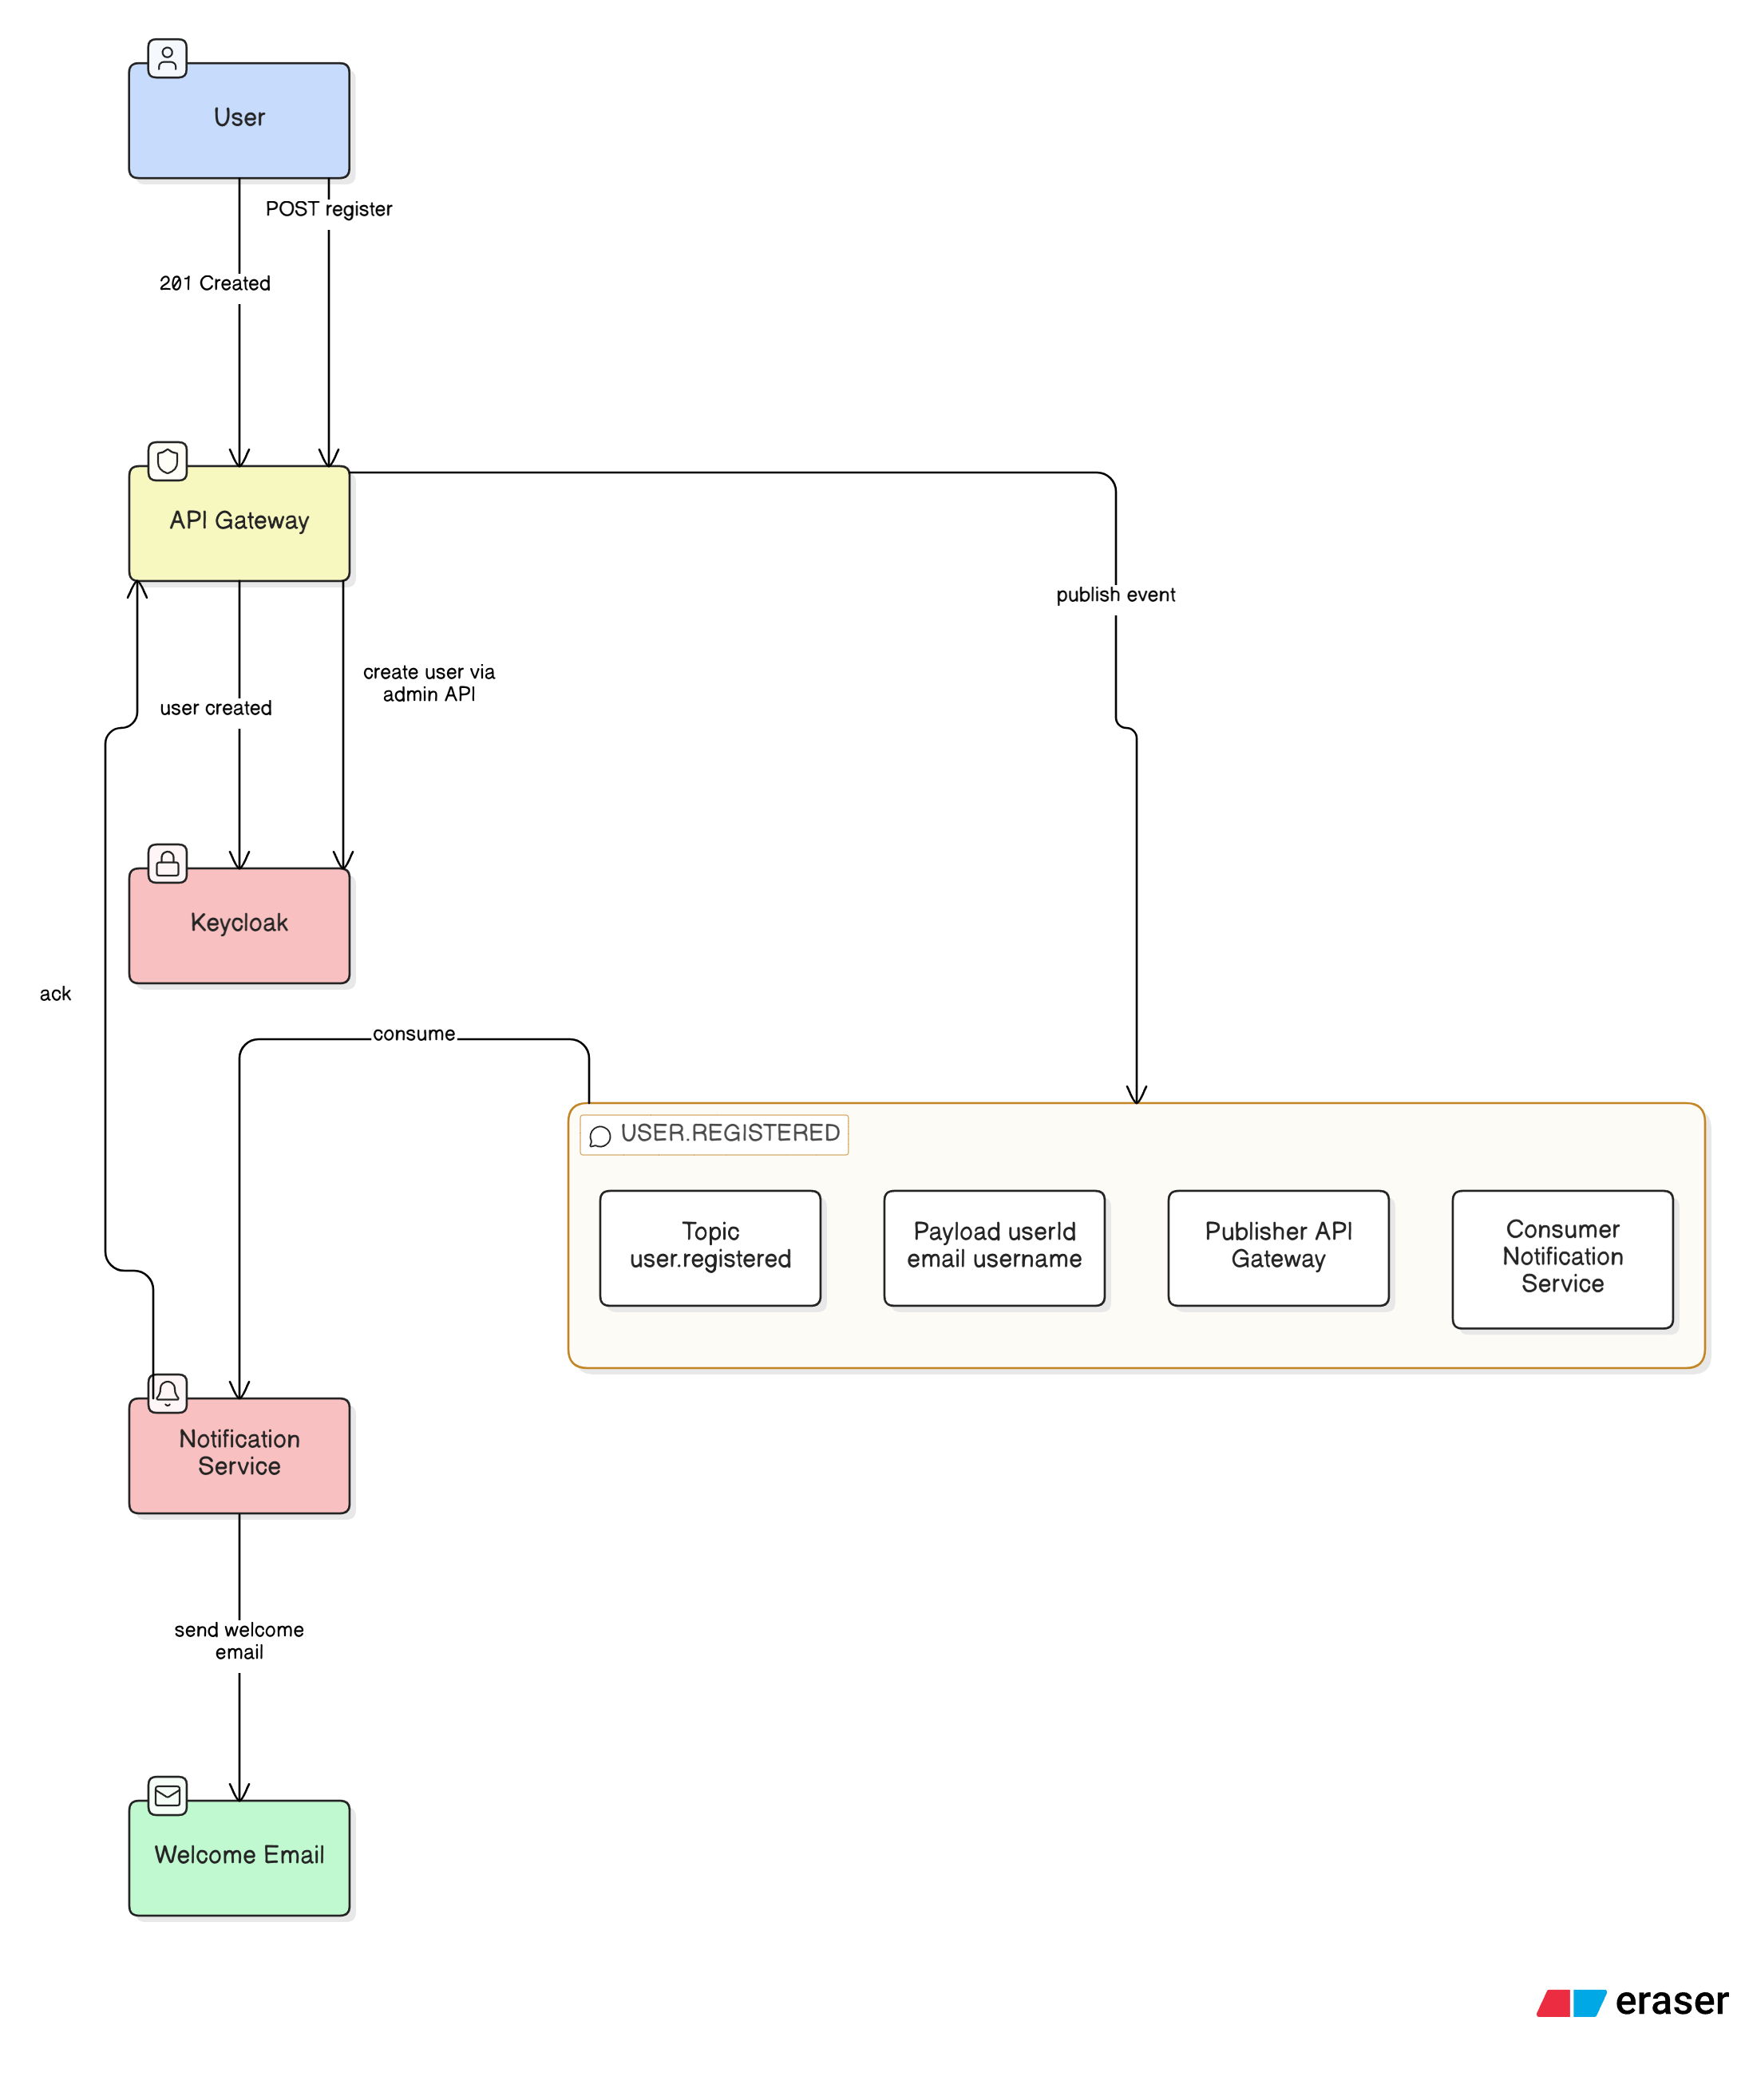
\includegraphics[width=0.8\textwidth]{images/user-created-event-flow.png}
\caption{Flux des événements Kafka — Publications et consommations}
\label{fig:event-flow}
\end{figure}

Les topics Kafka utilisés dans le projet sont visibles dans la capture ci-dessous.

\begin{figure}[H]
\centering
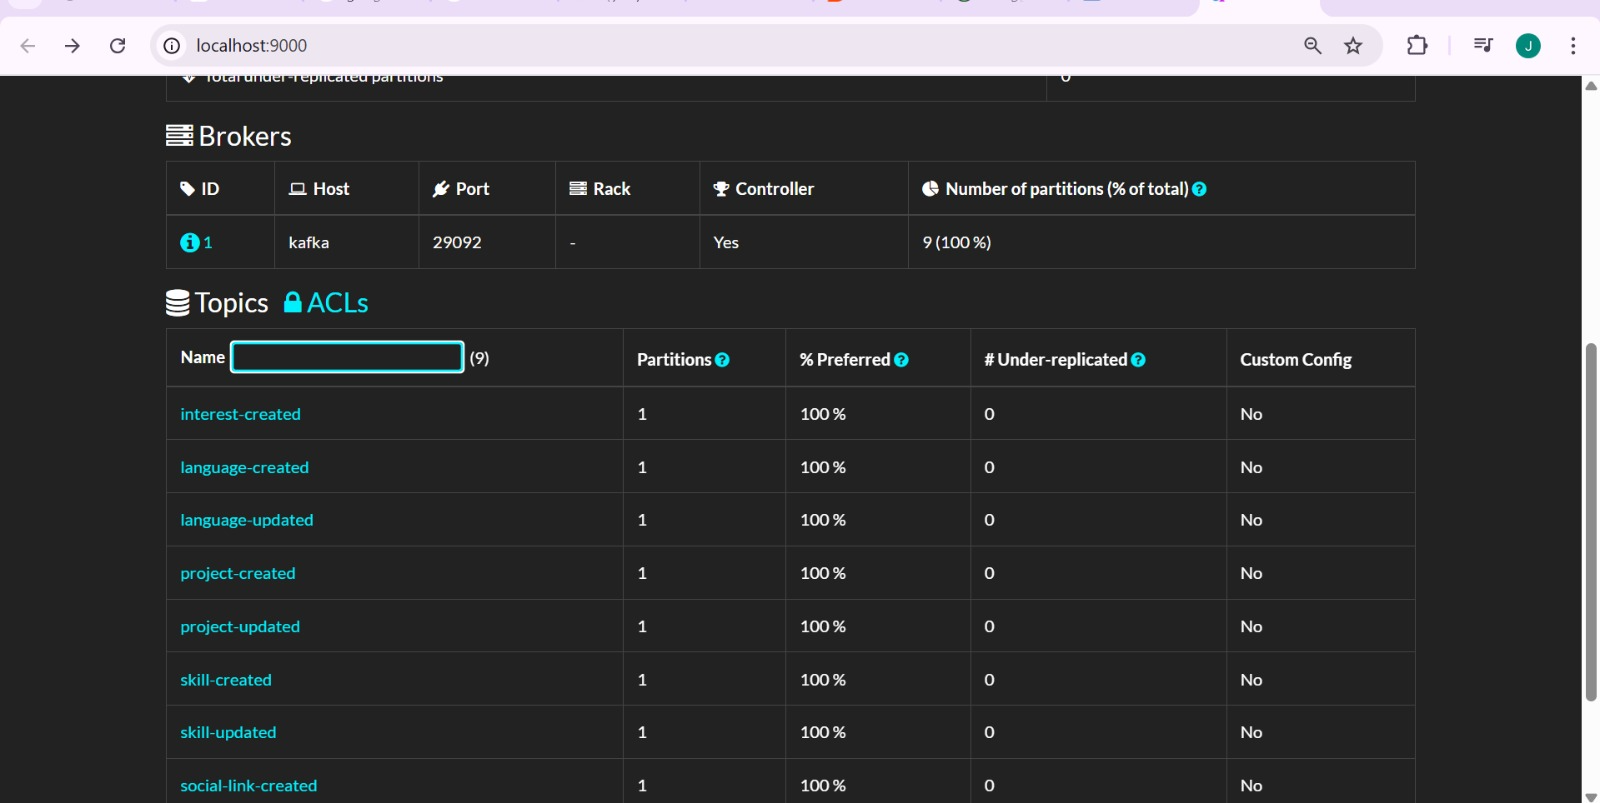
\includegraphics[width=0.8\textwidth]{images/kafka-topics.png}
\caption{Topics Kafka — user.registered, user.created, trigger-live-crawl}
\label{fig:kafka-topics}
\end{figure}

\subsection{Pipeline de génération de CV}
\label{subsec:realisation:pipeline-cv}

Le \textbf{Workflow Service} orchestre le pipeline de génération de CV, composé de 5 agents IA agissant en séquence. Chaque agent traite une étape spécifique du flux de travail.

\begin{figure}[H]
\centering
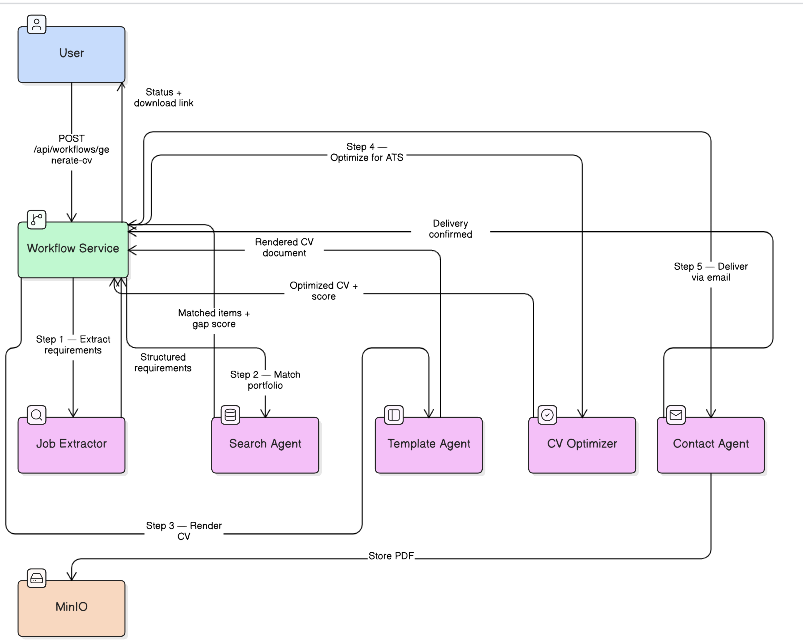
\includegraphics[width=\textwidth]{images/cv-generation-flow.png}
\caption{ Pipeline de génération de CV — De l'offre d'emploi à l'envoi par email}
\label{fig:pipeline-cv}
\end{figure}

\subsection{Développement Frontend}
\label{subsec:realisation:frontend}

Le frontend est développé avec \textbf{Angular 21} en utilisant les \textbf{standalone components}, \textbf{RxJS} pour la gestion asynchrone et les \textbf{Signals} pour la réactivité. L'interface suit le design system \textbf{Propel} avec des couleurs en espace OKLCH.

Les principales fonctionnalités du frontend incluent :
\begin{itemize}
    \item Pages de connexion et d'inscription (Keycloak).
    \item Tableau de bord avec statistiques et graphiques.
    \pagebreak
    \item Interface de génération de CV (saisie d'offre d'emploi).
    \item Vue Kanban pour le suivi des candidatures (drag-and-drop).
    \item Vue calendrier avec rappels.
    \item Gestion complète du portfolio.
    \item Vues liste et analytique des candidatures.
\end{itemize}

\subsection{Base de données}
\label{subsec:realisation:bdd}

L'architecture microservices implique l'utilisation de 8 bases de données \textbf{PostgreSQL 16} indépendantes, une par microservice, plus une pour Keycloak. Chaque base utilise l'extension \textbf{pgvector} pour le support des recherches vectorielles utilisées par l'agent de matching RAG.

\subsection{Documentation des API}
\label{subsec:realisation:api}

Chaque microservice expose ses endpoints via une interface \textbf{Swagger UI} intégrée, facilitant le test et la documentation des API. Les captures ci-dessous présentent la documentation de chaque service.

\begin{figure}[H]
\centering
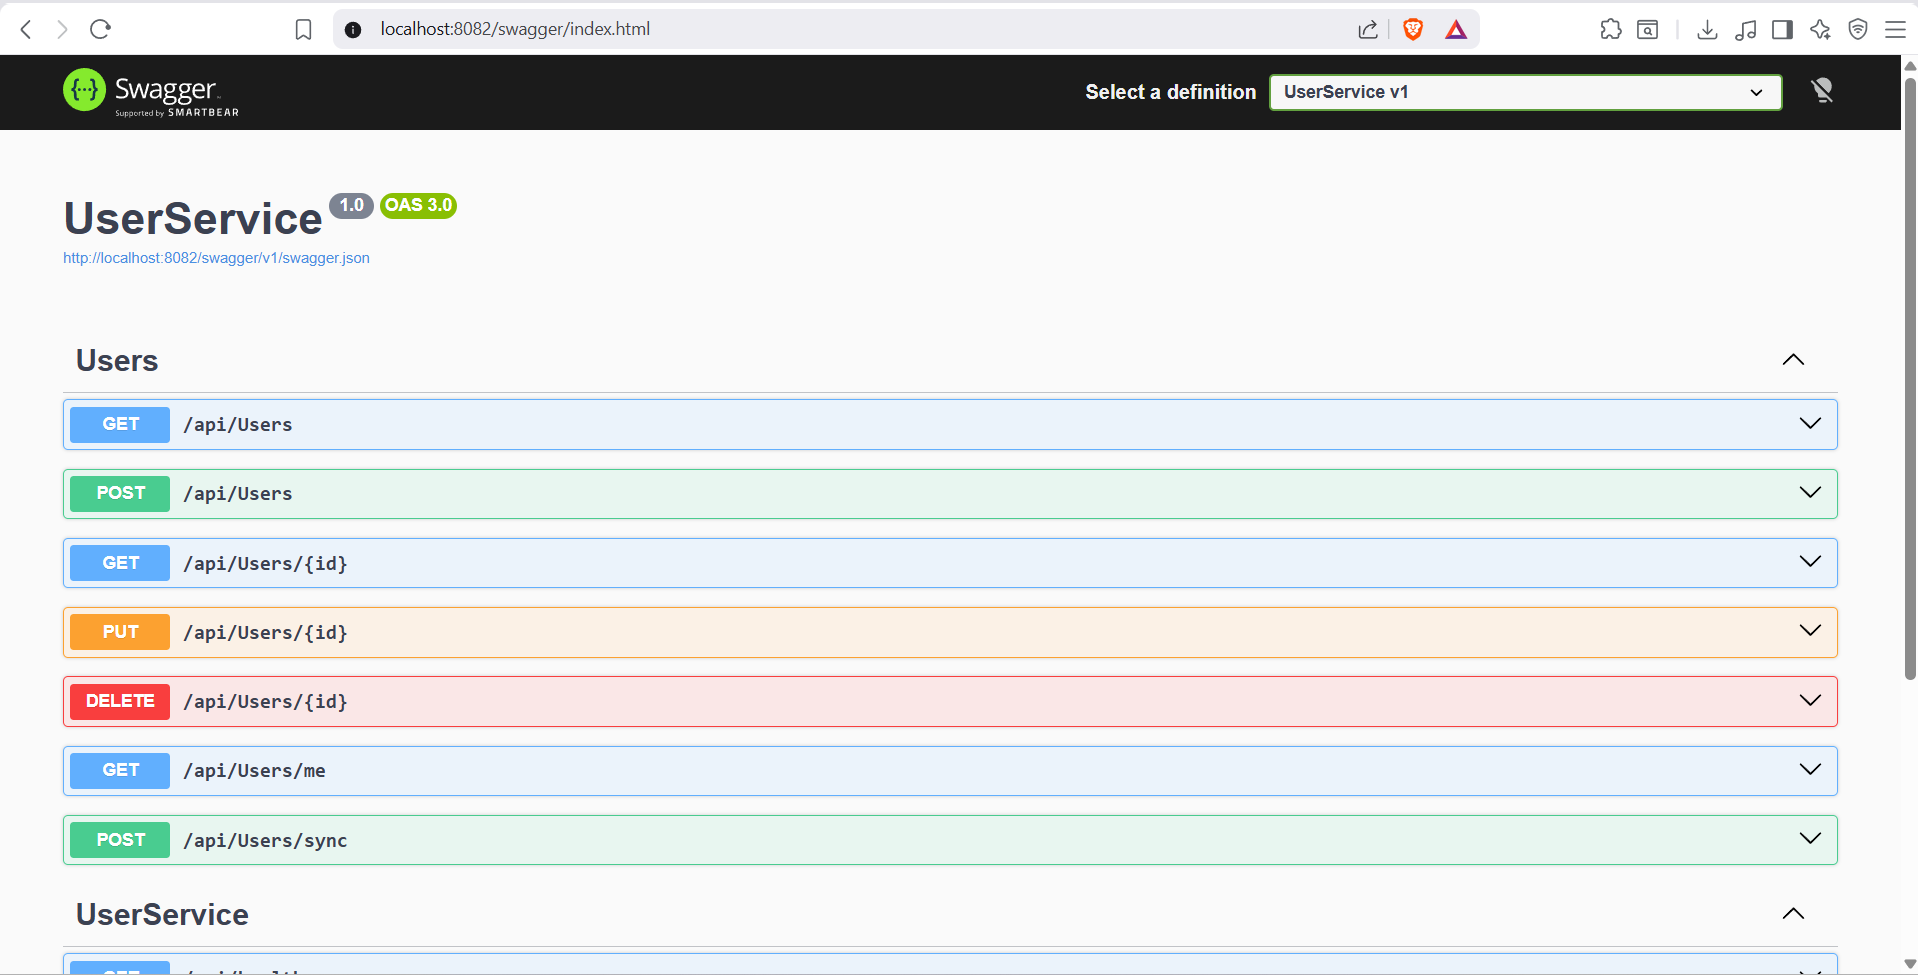
\includegraphics[width=0.49\textwidth]{images/swagger/user-service.png}
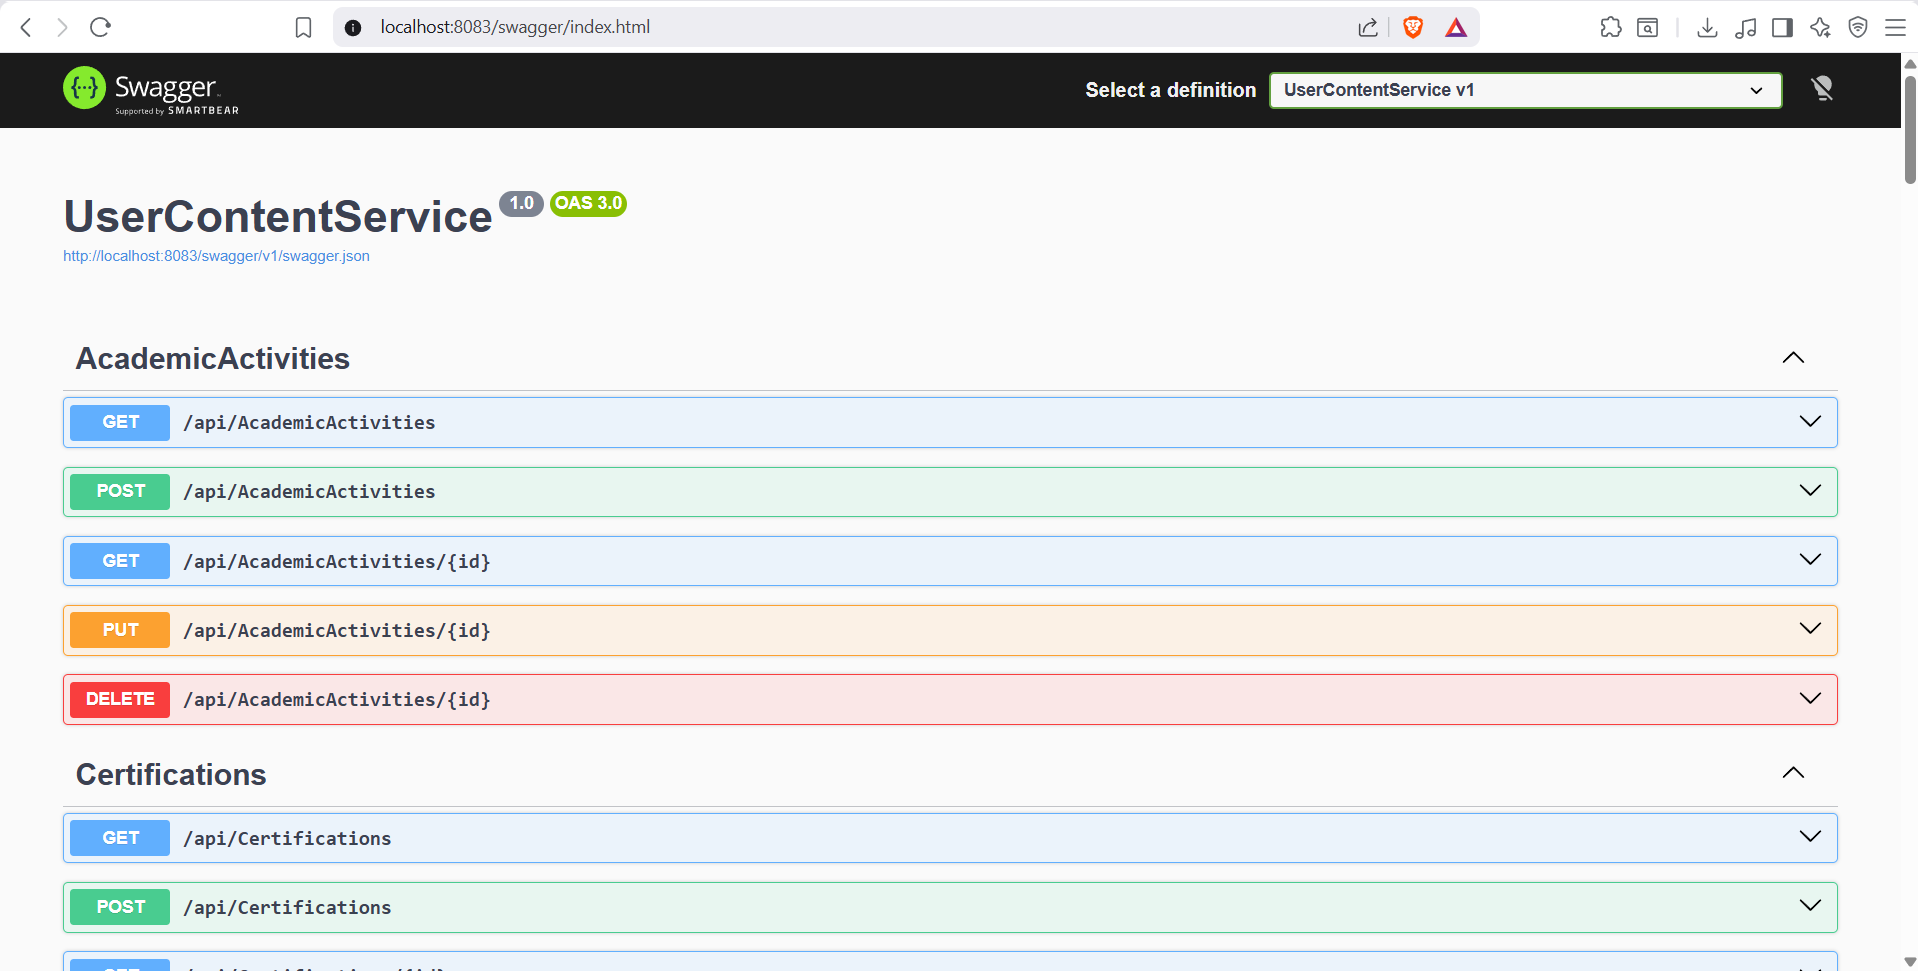
\includegraphics[width=0.49\textwidth]{images/swagger/user-content-service.png}
\caption{Documentation Swagger — User Service et User Content Service}
\label{fig:swagger-user}
\end{figure}

\begin{figure}[H]
\centering
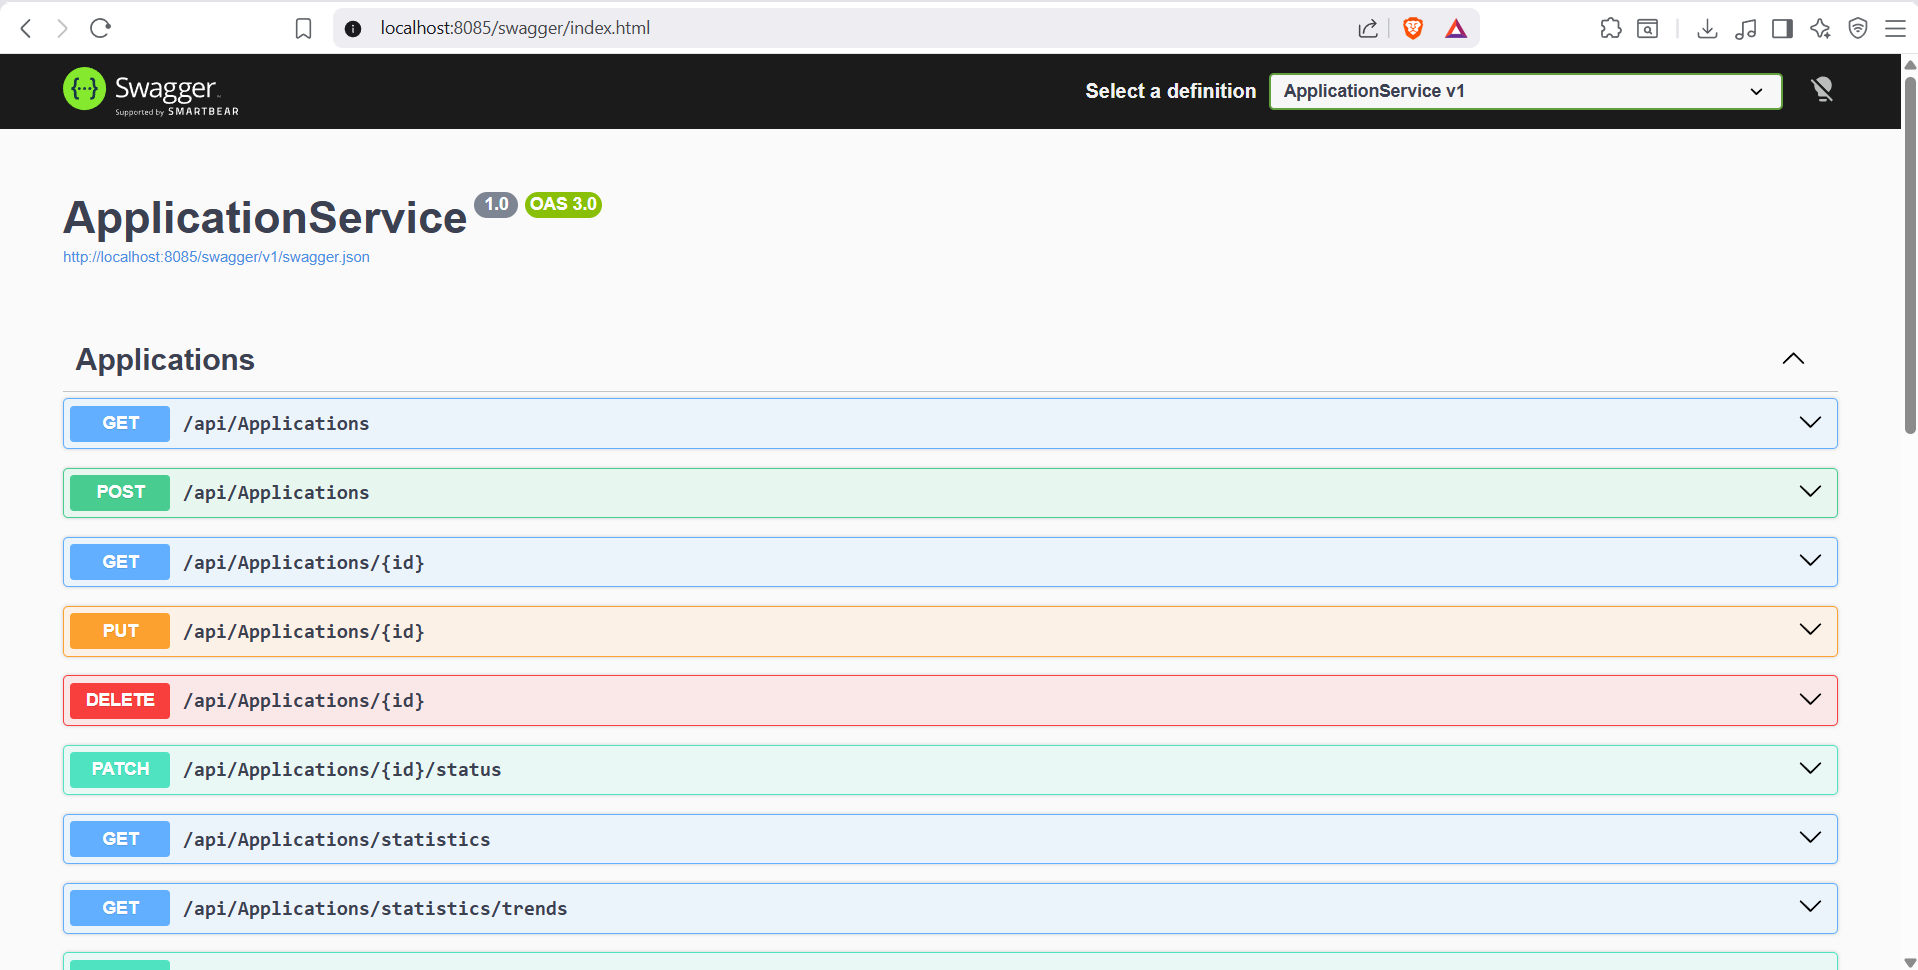
\includegraphics[width=0.49\textwidth]{images/swagger/application-service.png}
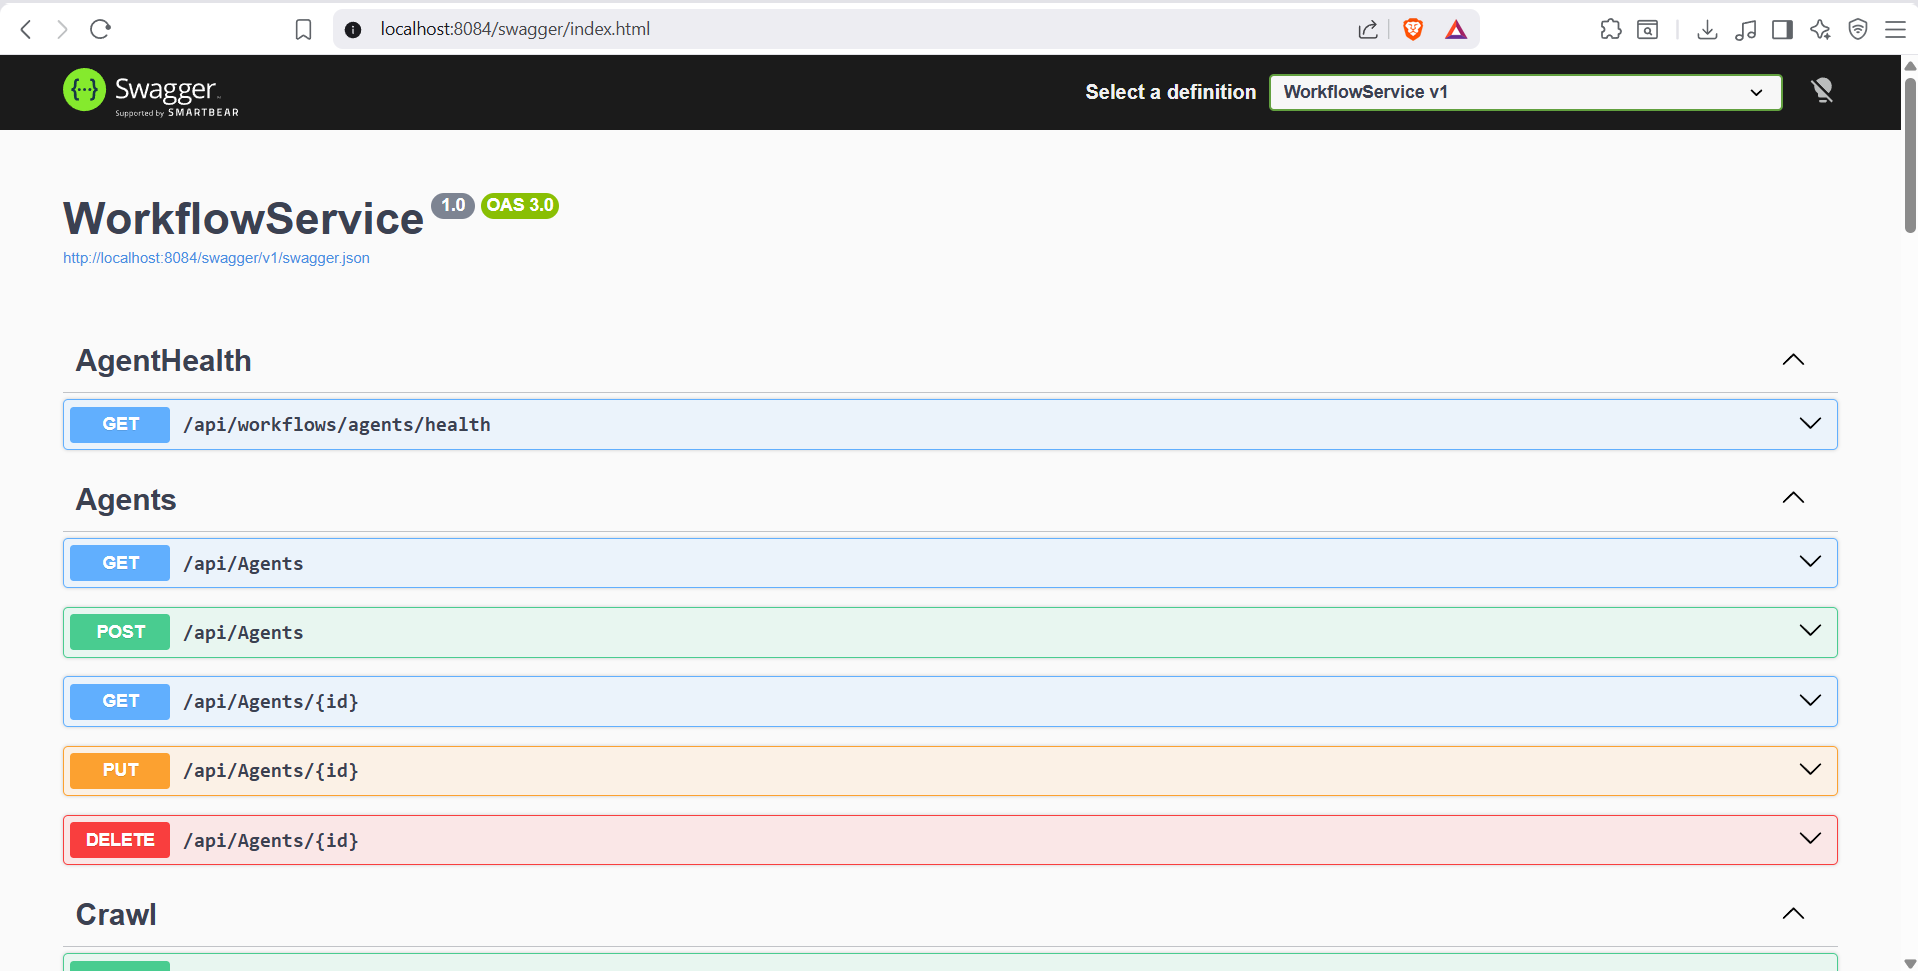
\includegraphics[width=0.49\textwidth]{images/swagger/workflow-service.png}
\caption{Documentation Swagger — Application Service et Workflow Service}
\label{fig:swagger-app-workflow}
\end{figure}

\begin{figure}[H]
\centering
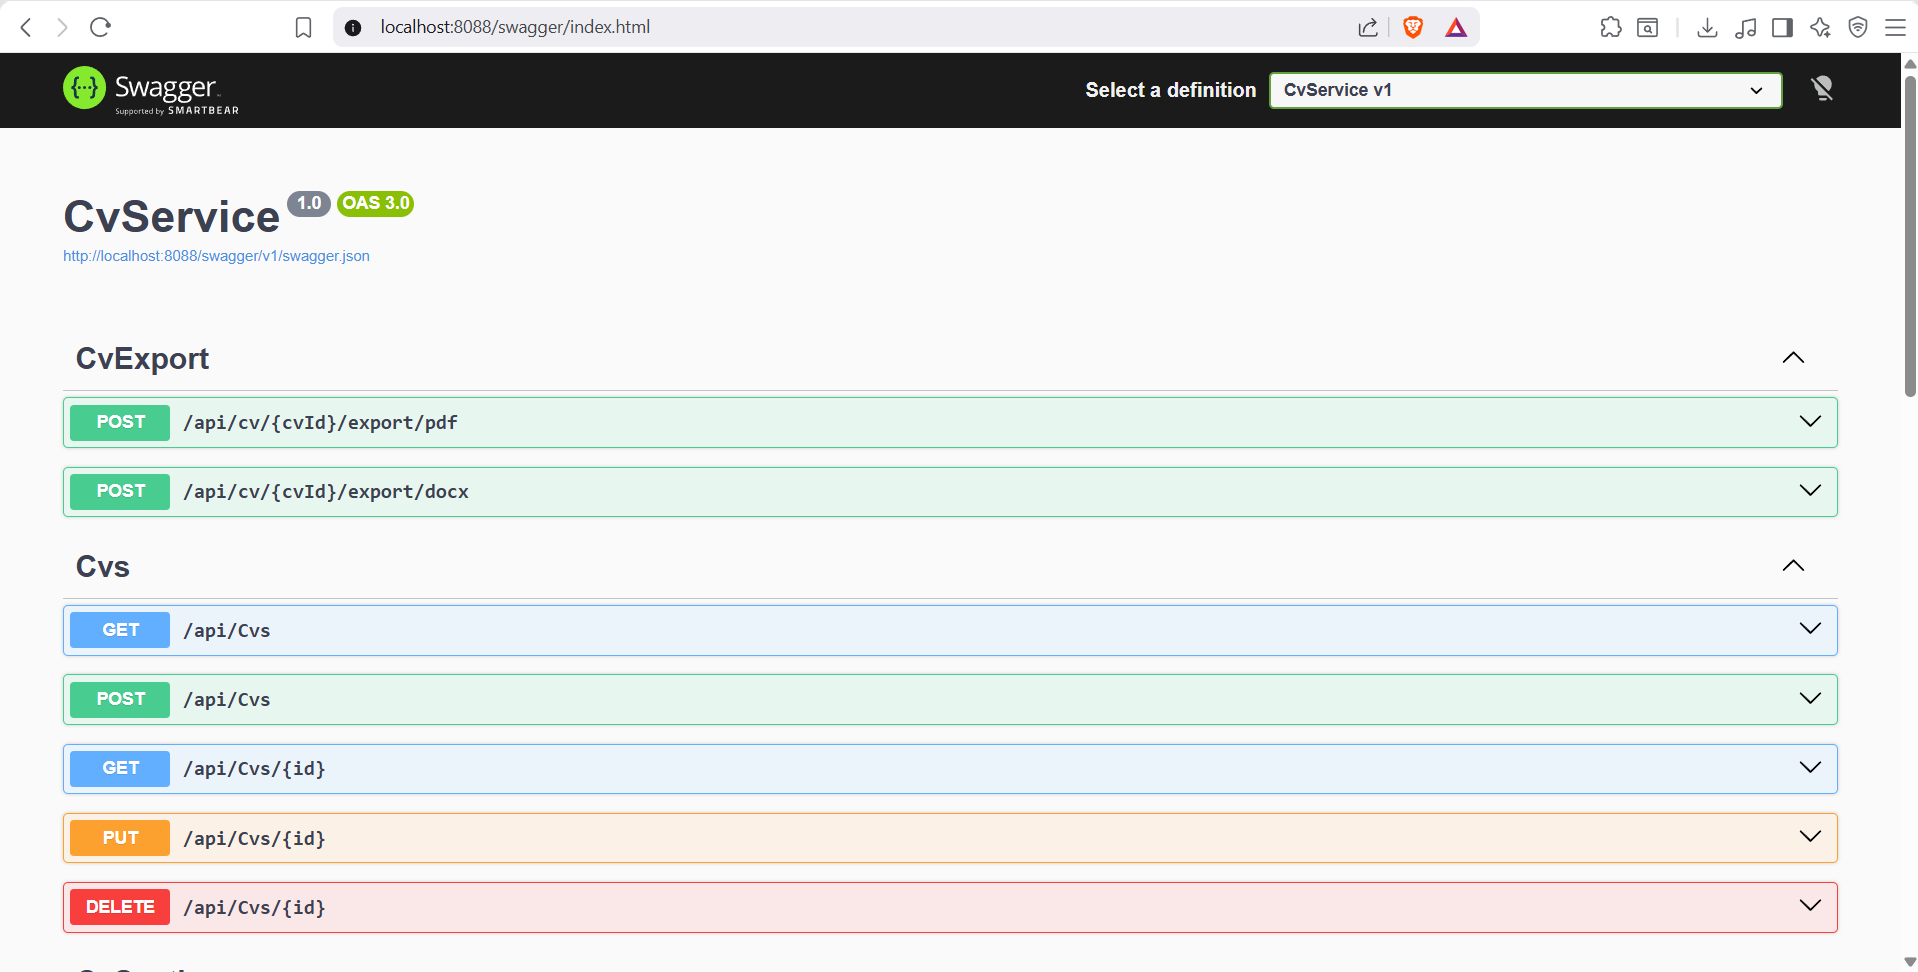
\includegraphics[width=0.49\textwidth]{images/swagger/cv-service.png}
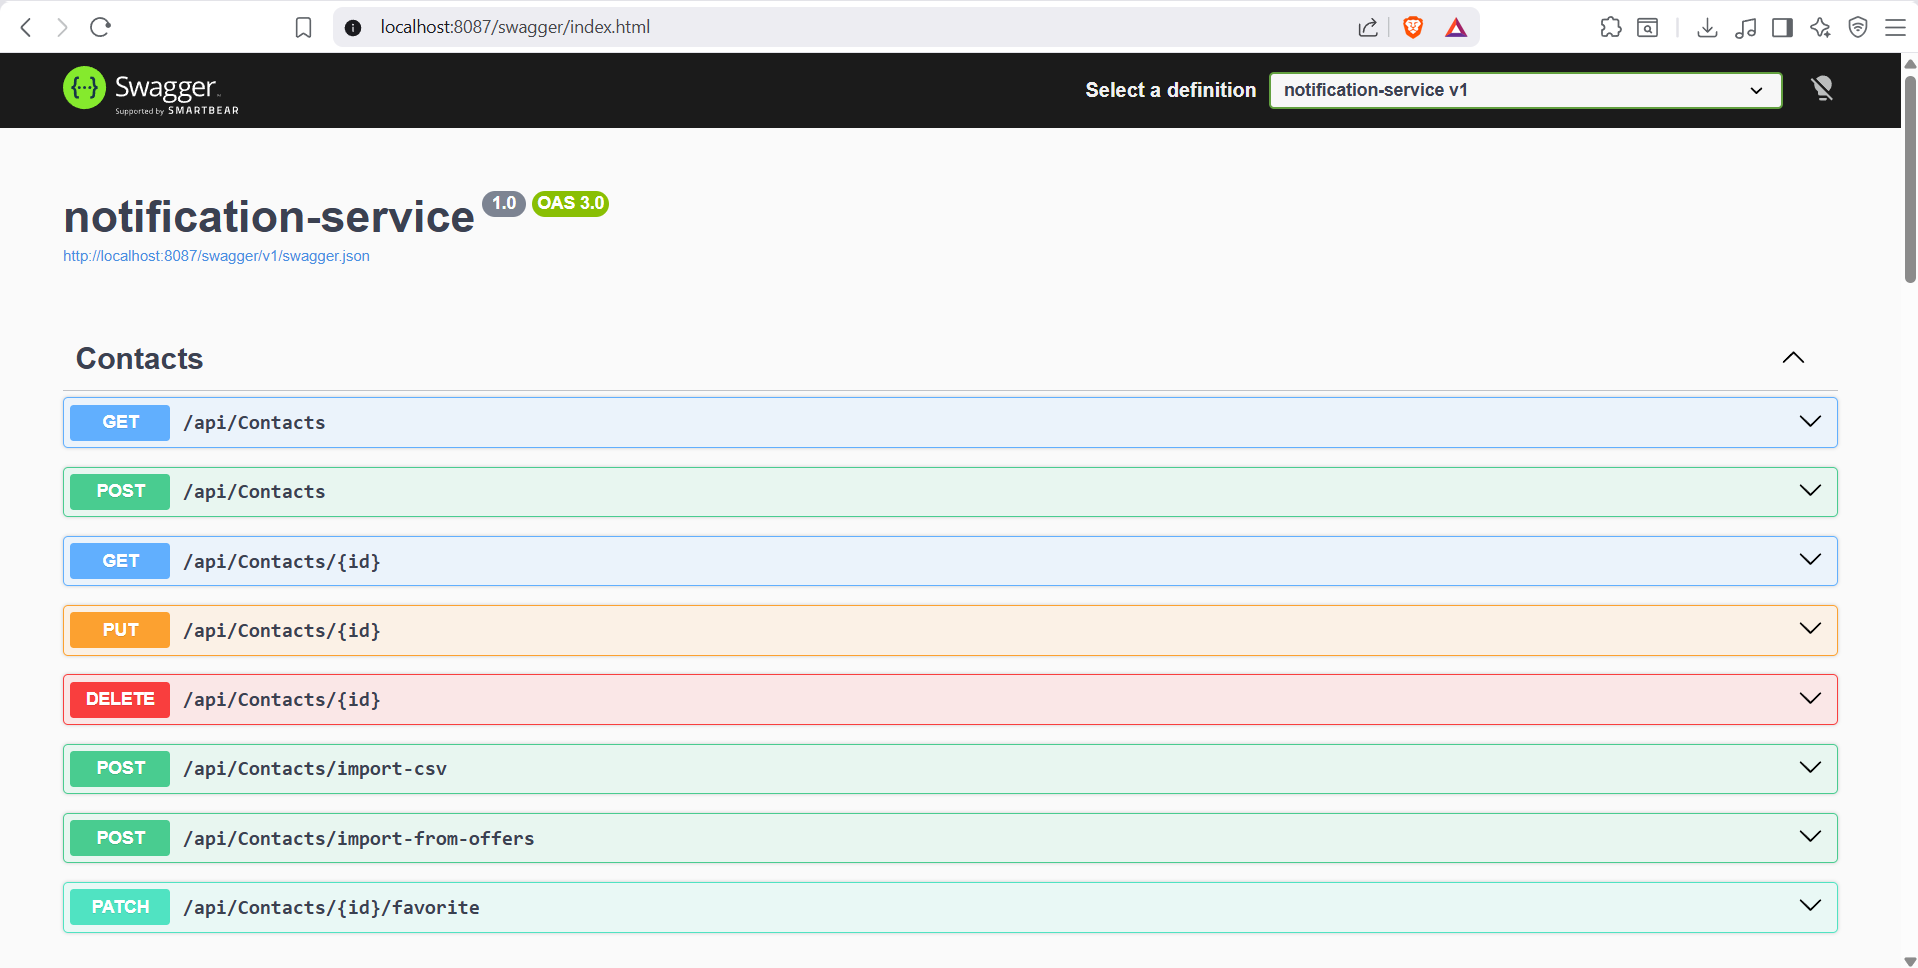
\includegraphics[width=0.49\textwidth]{images/swagger/notification-service.png}
\caption{Documentation Swagger — CV Service et Notification Service}
\label{fig:swagger-cv-notif}
\end{figure}

\begin{figure}[H]
\centering
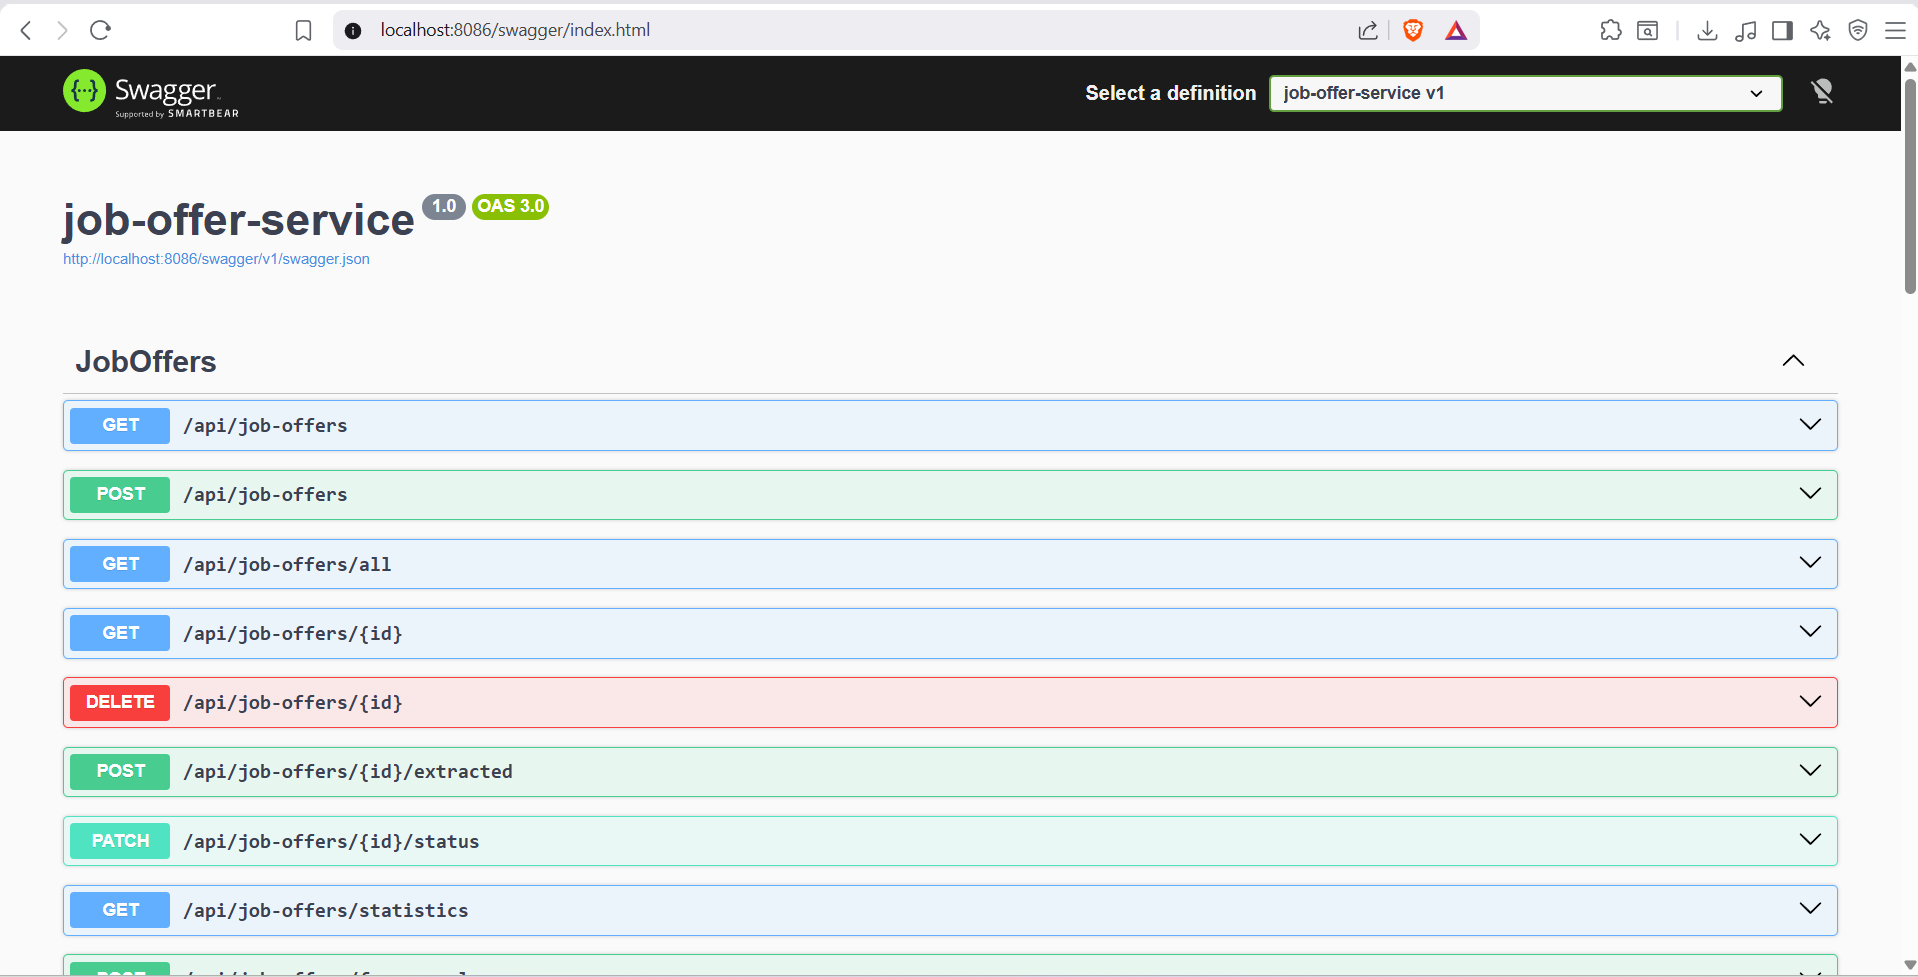
\includegraphics[width=0.49\textwidth]{images/swagger/job-offer-service.png}
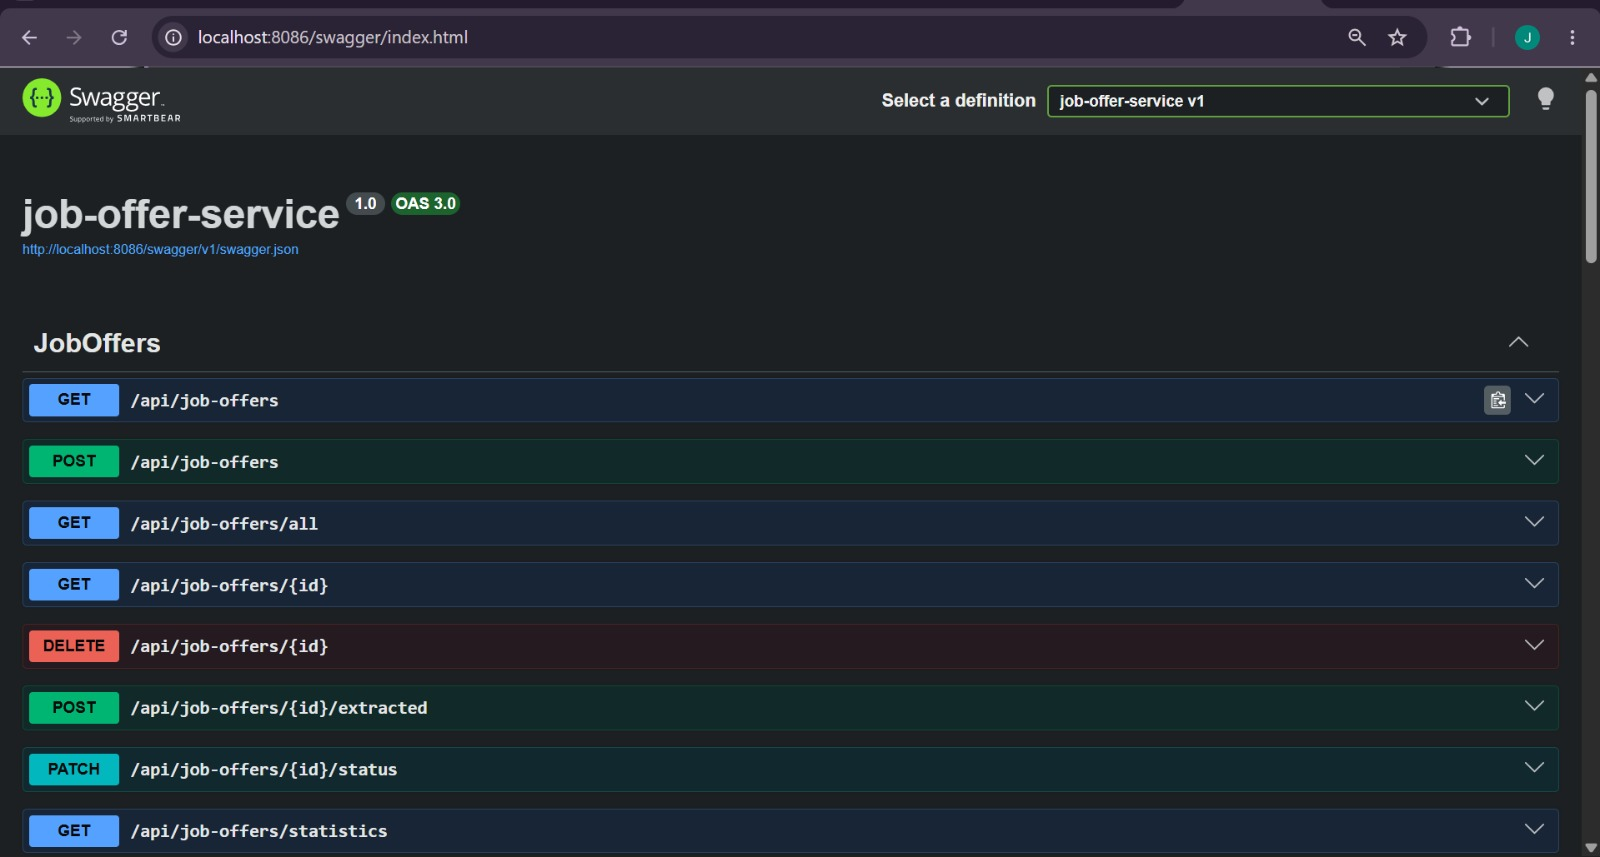
\includegraphics[width=0.49\textwidth]{images/swagger/job-offer-service1.png}
\caption{Documentation Swagger — Job Offer Service}
\label{fig:swagger-joboffer}
\end{figure}

\begin{figure}[H]
\centering
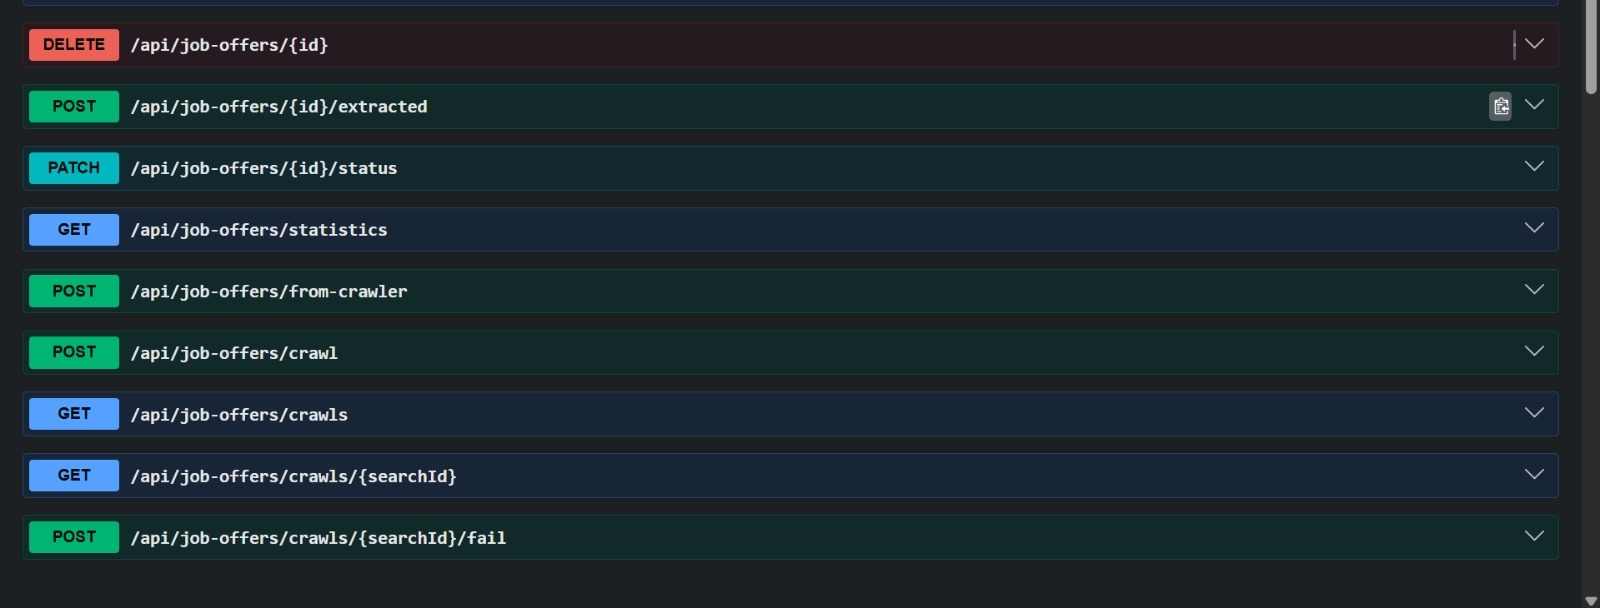
\includegraphics[width=0.49\textwidth]{images/swagger/job-offer-service2.png}
\caption{Documentation Swagger — Job Offer Service (suite)}
\label{fig:swagger-joboffer2}
\end{figure}

\section{Déploiement}
\label{sec:realisation:deploiement}

\subsection{Mise en place de l'environnement de développement}
\label{subsec:realisation:env-dev}

L'environnement de développement est entièrement conteneurisé. Un fichier \texttt{Makefile} à la racine du projet automatise les commandes courantes (démarrage des services, exécution des migrations, lancement des tests). Chaque sous-projet (backend, ai\_agents) possède également son propre Makefile.

\subsection{Dockerisation de l'application}
\label{subsec:realisation:docker}

L'ensemble de l'application est dockerisé avec des \textbf{Dockerfiles multi-stage} pour optimiser la taille des images de production. Au total, 18 Dockerfiles ont été créés couvrant l'ensemble des services.

Les images sont construites en deux étapes :
\begin{enumerate}
    \item \textbf{Build :} Compilation et génération des artefacts.
    \item \textbf{Runtime :} Image légère ne contenant que l'exécutable et ses dépendances.
\end{enumerate}

\begin{figure}[H]
\centering
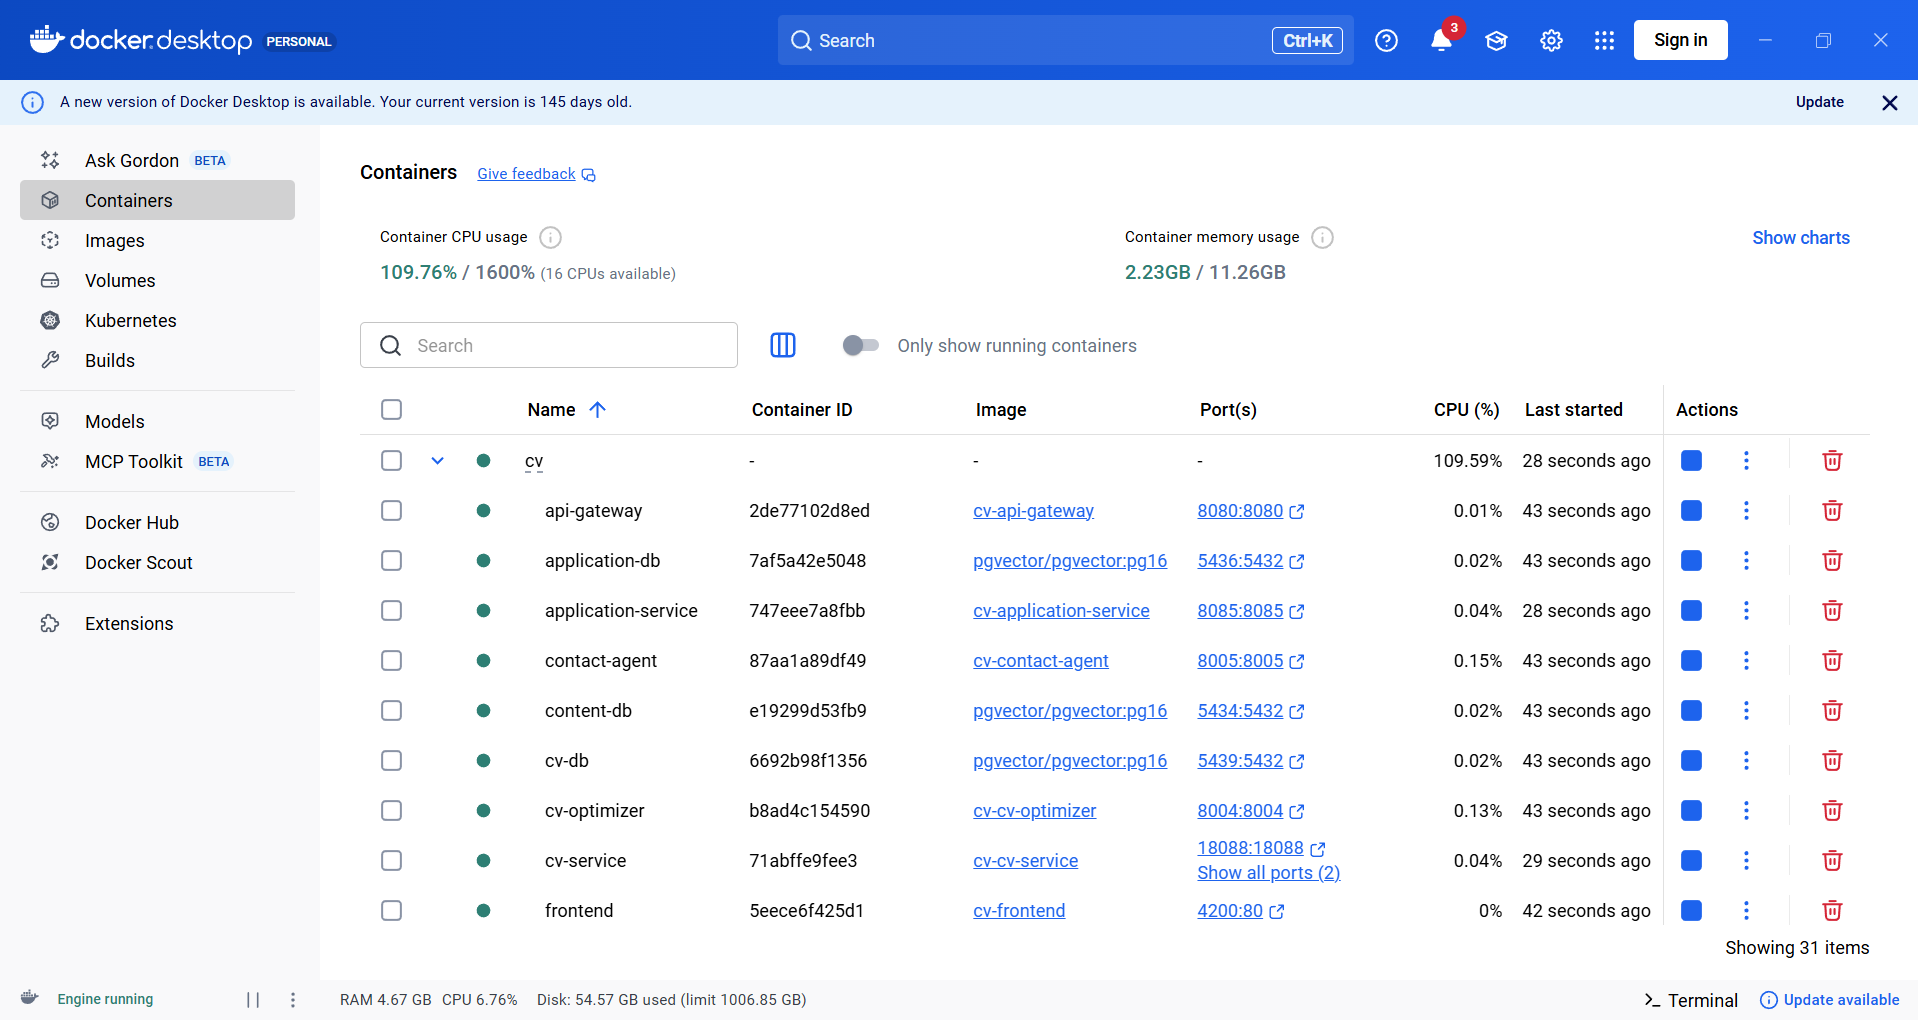
\includegraphics[width=0.85\textwidth]{images/docker-desktop-container-running.png}
\caption{Conteneurs Docker en cours d'exécution}
\label{fig:docker-containers}
\end{figure}

\subsection{Pipeline CI/CD}
\label{subsec:realisation:pipeline}

Le pipeline CI/CD est implémenté avec \textbf{GitHub Actions} et comprend 6 phases séquentielles. Chaque phase doit réussir pour passer à la suivante.

\begin{figure}[H]
\centering
% \includegraphics[width=\textwidth]{images/pipeline-cicd.png}
\caption{Pipeline CI/CD}
\label{fig:pipeline}
\end{figure}

\section{Présentation de l'application}
\label{sec:realisation:presentation}

\subsection{Interface utilisateur}
\label{subsec:realisation:ui}

\begin{figure}[H]
\centering
% \includegraphics[width=\textwidth]{images/screenshot-dashboard.png}
\caption{Interface du tableau de bord}
\label{fig:dashboard}
\end{figure}

\begin{figure}[H]
\centering
% \includegraphics[width=\textwidth]{images/screenshot-generation.png}
\caption{Interface de génération de CV}
\label{fig:generation}
\end{figure}

\begin{figure}[H]
\centering
% \includegraphics[width=\textwidth]{images/screenshot-kanban.png}
\caption{Tableau Kanban de suivi des candidatures}
\label{fig:kanban}
\end{figure}

\begin{figure}[H]
\centering
% \includegraphics[width=\textwidth]{images/screenshot-portfolio.png}
\caption{Interface de gestion du portfolio}
\label{fig:portfolio}
\end{figure}

\subsection{Fonctionnalités principales}
\label{subsec:realisation:fonctionnalites}

Le système \projectname{} offre les fonctionnalités principales suivantes :

\begin{itemize}
    \item \textbf{Génération intelligente de CV :} Pipeline de 6 agents IA (extraction, matching RAG, template, optimisation ATS, contact) coordonnés par un orchestrateur.
    \item \textbf{Suivi de candidatures :} Vue Kanban avec drag-and-drop, vue liste, vue calendrier, graphiques analytiques.
    \item \textbf{Gestion de portfolio :} CRUD complet pour projets, compétences, expériences, formations, certifications, langues et réseaux sociaux.
    \item \textbf{Crawling d'offres d'emploi :} Agent IA dédié qui collecte automatiquement les offres depuis des plateformes externes.
    \item \textbf{Notifications temps réel :} SignalR pour les mises à jour en direct, Hangfire pour les rappels planifiés, emails via MailKit.
\end{itemize}

\subsection{Démonstrations du fonctionnement}
\label{subsec:realisation:demo}

% À remplir : description des démonstrations du fonctionnement de l'application

\section{Conclusion}
\label{sec:realisation:conclusion}

Ce chapitre a présenté en détail la réalisation technique du projet \projectname{}. Nous avons couvert l'architecture physique et logicielle, les outils utilisés, le cycle DevSecOps, la gestion du code source, l'implémentation des différentes couches et le déploiement. Le projet démontre une maîtrise complète de la chaîne DevOps, de l'écriture du code jusqu'au déploiement automatisé en passant par la sécurité et la qualité.
